\documentclass[10pt,a4paper]{article}
\usepackage[margin=1.8cm]{geometry}
\usepackage[T1]{fontenc}
\usepackage{lmodern,amsmath,amssymb,booktabs,microtype,tikz,pgfplots}
\usepackage[font=small,labelfont=bf,skip=2pt,hypcap=false]{caption}
\usepackage[hidelinks]{hyperref}
\pgfplotsset{compat=1.18}
\setlength{\parindent}{0pt}
\setlength{\parskip}{2pt}
\newcommand{\heading}[1]{\par\medskip\noindent{\large\bfseries #1}\par}
\newcommand{\StartDate}{2021-10-11}
\newcommand{\EndDate}{2026-10-08}
\newcommand{\PriceDays}{1254}
\newcommand{\ReturnDays}{1253}
\newcommand{\SplitDate}{2024-10-11}
\newcommand{\InDays}{755}
\newcommand{\OutDays}{498}
\newcommand{\FullDen}{2.591}
\newcommand{\FullInterpretation}{The unrestricted tangency has 94.59\% fitted log-proxy return, 59.46\% volatility and gross exposure 16.93 times equity. Its largest position is 683.31\% in SPY. These weights require substantial shorting and are not an investable recommendation. The long-only tangency instead combines 44.75\% SPY and 55.25\% GLD, with proxy Sharpe 0.868. The long-only MVP has volatility 5.90\%, versus 3.45\% unrestricted.}
\newcommand{\ISDiagnostic}{On the training sample, $d=-2.475<0$. Thus there is no finite fully invested unrestricted Sharpe maximum. Its supremum is $\sqrt{C-B^2/A}=1.901$, approached only with unbounded leverage; the normalized closed form is a Sharpe minimum, not a tangency maximum. The extra bounded diagnostic imposes $|w_i|\le3$ and solves a different problem. It is labeled separately and does not replace the unavailable unrestricted optimum.}
\newcommand{\OOSInterpretation}{The long-only tangency earns Sharpe 1.052 versus 0.796 for equal weight, with total gains of 51.00\% and 25.57\%, respectively. Its maximum drawdown is -17.50\% versus -10.54\%. The bounded diagnostic earns 1.060 Sharpe but draws down -46.32\%. Both MVPs reduce volatility but underperform the benchmark in Sharpe. Higher realized return therefore does not imply safer implementation.}

\begin{document}
\begin{center}
{\Large\bfseries Mean--Variance Optimization of Ten ETFs}\\[4pt]
{\small Assignment 1: empirical analysis and chronological robustness}\\[4pt]
{\small Wei Qi \quad \href{mailto:226010267@link.cuhk.edu.cn}{226010267@link.cuhk.edu.cn}}
\end{center}
\heading{1. Data and estimation}
The universe spans US equity (SPY, QQQ, IWM), international equity (EFA, EEM), aggregate bonds (AGG), long Treasuries (TLT), high-yield credit (HYG), gold (GLD), and US real estate (VNQ). The supplied Yahoo Finance adjusted-close snapshot covers \StartDate{}--\EndDate{}, with \PriceDays{} prices and \ReturnDays{} daily return observations per ETF. There are no missing prices in the analysis panel. Adjustments account for splits and distributions; USD prices describe US-listed instruments, not exclusively US economic exposures.

For daily log returns $\ell_{it}=\log(P_{it}/P_{i,t-1})$, the estimates are
\[
\widehat\mu=m\bar\ell,\qquad \widehat\Sigma=m\frac{\sum_t(\ell_t-\bar\ell)(\ell_t-\bar\ell)^\top}{T-1},\qquad m=252.
\]
The annualized mean standard error under independent observations is $m s_i/\sqrt T$, not annualized volatility divided by $\sqrt T$. Dependence would require a HAC estimator or block bootstrap. The table reports log means and volatilities; $e^{\widehat\mu_i}-1$ is historical annualized geometric growth, not an expected arithmetic return.
\begin{center}
\begin{minipage}[t]{0.51\textwidth}\centering\vspace{0pt}\small
\captionof{table}{Annualized ETF log-return estimates.}
\begin{tabular}{lrrr}\toprule
ETF & Log mean (\%) & Vol. (\%) & Mean SE (\%)\\\midrule
SPY & 12.91 & 17.12 & 7.68 \\
QQQ & 15.37 & 22.95 & 10.29 \\
IWM & 5.81 & 22.35 & 10.02 \\
EFA & 8.71 & 16.60 & 7.45 \\
EEM & 7.62 & 19.98 & 8.96 \\
AGG & -0.44 & 6.14 & 2.75 \\
TLT & -8.45 & 15.68 & 7.03 \\
HYG & 3.36 & 7.54 & 3.38 \\
GLD & 16.83 & 19.00 & 8.52 \\
VNQ & 0.91 & 18.86 & 8.46
\\\bottomrule
\end{tabular}
\end{minipage}\hfill
\begin{minipage}[t]{0.46\textwidth}\centering\vspace{0pt}
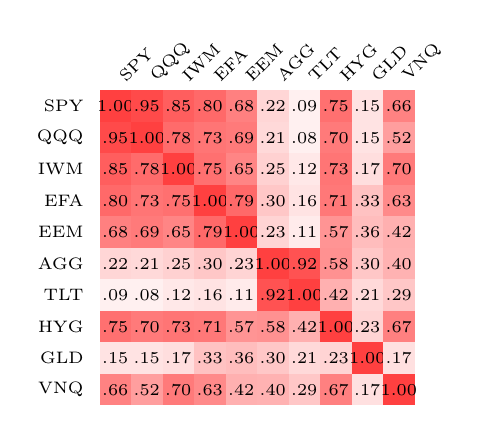
\begin{tikzpicture}[x=0.40cm,y=0.40cm,every node/.style={font=\fontsize{6}{7}\selectfont}]
\node[anchor=east] at (-.2,-0.5) {SPY};
\node[rotate=45,anchor=west] at (0.5,.15) {SPY};
\fill[red!75!white] (0,0) rectangle ++(1,-1);
\node at (0.5,-0.5) {1.00};
\fill[red!71!white] (1,0) rectangle ++(1,-1);
\node at (1.5,-0.5) {.95};
\fill[red!63!white] (2,0) rectangle ++(1,-1);
\node at (2.5,-0.5) {.85};
\fill[red!59!white] (3,0) rectangle ++(1,-1);
\node at (3.5,-0.5) {.80};
\fill[red!50!white] (4,0) rectangle ++(1,-1);
\node at (4.5,-0.5) {.68};
\fill[red!16!white] (5,0) rectangle ++(1,-1);
\node at (5.5,-0.5) {.22};
\fill[red!6!white] (6,0) rectangle ++(1,-1);
\node at (6.5,-0.5) {.09};
\fill[red!56!white] (7,0) rectangle ++(1,-1);
\node at (7.5,-0.5) {.75};
\fill[red!11!white] (8,0) rectangle ++(1,-1);
\node at (8.5,-0.5) {.15};
\fill[red!49!white] (9,0) rectangle ++(1,-1);
\node at (9.5,-0.5) {.66};
\node[anchor=east] at (-.2,-1.5) {QQQ};
\node[rotate=45,anchor=west] at (1.5,.15) {QQQ};
\fill[red!71!white] (0,-1) rectangle ++(1,-1);
\node at (0.5,-1.5) {.95};
\fill[red!75!white] (1,-1) rectangle ++(1,-1);
\node at (1.5,-1.5) {1.00};
\fill[red!58!white] (2,-1) rectangle ++(1,-1);
\node at (2.5,-1.5) {.78};
\fill[red!54!white] (3,-1) rectangle ++(1,-1);
\node at (3.5,-1.5) {.73};
\fill[red!52!white] (4,-1) rectangle ++(1,-1);
\node at (4.5,-1.5) {.69};
\fill[red!15!white] (5,-1) rectangle ++(1,-1);
\node at (5.5,-1.5) {.21};
\fill[red!6!white] (6,-1) rectangle ++(1,-1);
\node at (6.5,-1.5) {.08};
\fill[red!52!white] (7,-1) rectangle ++(1,-1);
\node at (7.5,-1.5) {.70};
\fill[red!11!white] (8,-1) rectangle ++(1,-1);
\node at (8.5,-1.5) {.15};
\fill[red!38!white] (9,-1) rectangle ++(1,-1);
\node at (9.5,-1.5) {.52};
\node[anchor=east] at (-.2,-2.5) {IWM};
\node[rotate=45,anchor=west] at (2.5,.15) {IWM};
\fill[red!63!white] (0,-2) rectangle ++(1,-1);
\node at (0.5,-2.5) {.85};
\fill[red!58!white] (1,-2) rectangle ++(1,-1);
\node at (1.5,-2.5) {.78};
\fill[red!75!white] (2,-2) rectangle ++(1,-1);
\node at (2.5,-2.5) {1.00};
\fill[red!56!white] (3,-2) rectangle ++(1,-1);
\node at (3.5,-2.5) {.75};
\fill[red!48!white] (4,-2) rectangle ++(1,-1);
\node at (4.5,-2.5) {.65};
\fill[red!18!white] (5,-2) rectangle ++(1,-1);
\node at (5.5,-2.5) {.25};
\fill[red!9!white] (6,-2) rectangle ++(1,-1);
\node at (6.5,-2.5) {.12};
\fill[red!54!white] (7,-2) rectangle ++(1,-1);
\node at (7.5,-2.5) {.73};
\fill[red!13!white] (8,-2) rectangle ++(1,-1);
\node at (8.5,-2.5) {.17};
\fill[red!52!white] (9,-2) rectangle ++(1,-1);
\node at (9.5,-2.5) {.70};
\node[anchor=east] at (-.2,-3.5) {EFA};
\node[rotate=45,anchor=west] at (3.5,.15) {EFA};
\fill[red!59!white] (0,-3) rectangle ++(1,-1);
\node at (0.5,-3.5) {.80};
\fill[red!54!white] (1,-3) rectangle ++(1,-1);
\node at (1.5,-3.5) {.73};
\fill[red!56!white] (2,-3) rectangle ++(1,-1);
\node at (2.5,-3.5) {.75};
\fill[red!75!white] (3,-3) rectangle ++(1,-1);
\node at (3.5,-3.5) {1.00};
\fill[red!59!white] (4,-3) rectangle ++(1,-1);
\node at (4.5,-3.5) {.79};
\fill[red!22!white] (5,-3) rectangle ++(1,-1);
\node at (5.5,-3.5) {.30};
\fill[red!11!white] (6,-3) rectangle ++(1,-1);
\node at (6.5,-3.5) {.16};
\fill[red!53!white] (7,-3) rectangle ++(1,-1);
\node at (7.5,-3.5) {.71};
\fill[red!24!white] (8,-3) rectangle ++(1,-1);
\node at (8.5,-3.5) {.33};
\fill[red!46!white] (9,-3) rectangle ++(1,-1);
\node at (9.5,-3.5) {.63};
\node[anchor=east] at (-.2,-4.5) {EEM};
\node[rotate=45,anchor=west] at (4.5,.15) {EEM};
\fill[red!50!white] (0,-4) rectangle ++(1,-1);
\node at (0.5,-4.5) {.68};
\fill[red!52!white] (1,-4) rectangle ++(1,-1);
\node at (1.5,-4.5) {.69};
\fill[red!48!white] (2,-4) rectangle ++(1,-1);
\node at (2.5,-4.5) {.65};
\fill[red!59!white] (3,-4) rectangle ++(1,-1);
\node at (3.5,-4.5) {.79};
\fill[red!75!white] (4,-4) rectangle ++(1,-1);
\node at (4.5,-4.5) {1.00};
\fill[red!17!white] (5,-4) rectangle ++(1,-1);
\node at (5.5,-4.5) {.23};
\fill[red!8!white] (6,-4) rectangle ++(1,-1);
\node at (6.5,-4.5) {.11};
\fill[red!42!white] (7,-4) rectangle ++(1,-1);
\node at (7.5,-4.5) {.57};
\fill[red!26!white] (8,-4) rectangle ++(1,-1);
\node at (8.5,-4.5) {.36};
\fill[red!31!white] (9,-4) rectangle ++(1,-1);
\node at (9.5,-4.5) {.42};
\node[anchor=east] at (-.2,-5.5) {AGG};
\node[rotate=45,anchor=west] at (5.5,.15) {AGG};
\fill[red!16!white] (0,-5) rectangle ++(1,-1);
\node at (0.5,-5.5) {.22};
\fill[red!15!white] (1,-5) rectangle ++(1,-1);
\node at (1.5,-5.5) {.21};
\fill[red!18!white] (2,-5) rectangle ++(1,-1);
\node at (2.5,-5.5) {.25};
\fill[red!22!white] (3,-5) rectangle ++(1,-1);
\node at (3.5,-5.5) {.30};
\fill[red!17!white] (4,-5) rectangle ++(1,-1);
\node at (4.5,-5.5) {.23};
\fill[red!75!white] (5,-5) rectangle ++(1,-1);
\node at (5.5,-5.5) {1.00};
\fill[red!68!white] (6,-5) rectangle ++(1,-1);
\node at (6.5,-5.5) {.92};
\fill[red!43!white] (7,-5) rectangle ++(1,-1);
\node at (7.5,-5.5) {.58};
\fill[red!22!white] (8,-5) rectangle ++(1,-1);
\node at (8.5,-5.5) {.30};
\fill[red!30!white] (9,-5) rectangle ++(1,-1);
\node at (9.5,-5.5) {.40};
\node[anchor=east] at (-.2,-6.5) {TLT};
\node[rotate=45,anchor=west] at (6.5,.15) {TLT};
\fill[red!6!white] (0,-6) rectangle ++(1,-1);
\node at (0.5,-6.5) {.09};
\fill[red!6!white] (1,-6) rectangle ++(1,-1);
\node at (1.5,-6.5) {.08};
\fill[red!9!white] (2,-6) rectangle ++(1,-1);
\node at (2.5,-6.5) {.12};
\fill[red!11!white] (3,-6) rectangle ++(1,-1);
\node at (3.5,-6.5) {.16};
\fill[red!8!white] (4,-6) rectangle ++(1,-1);
\node at (4.5,-6.5) {.11};
\fill[red!68!white] (5,-6) rectangle ++(1,-1);
\node at (5.5,-6.5) {.92};
\fill[red!75!white] (6,-6) rectangle ++(1,-1);
\node at (6.5,-6.5) {1.00};
\fill[red!31!white] (7,-6) rectangle ++(1,-1);
\node at (7.5,-6.5) {.42};
\fill[red!15!white] (8,-6) rectangle ++(1,-1);
\node at (8.5,-6.5) {.21};
\fill[red!22!white] (9,-6) rectangle ++(1,-1);
\node at (9.5,-6.5) {.29};
\node[anchor=east] at (-.2,-7.5) {HYG};
\node[rotate=45,anchor=west] at (7.5,.15) {HYG};
\fill[red!56!white] (0,-7) rectangle ++(1,-1);
\node at (0.5,-7.5) {.75};
\fill[red!52!white] (1,-7) rectangle ++(1,-1);
\node at (1.5,-7.5) {.70};
\fill[red!54!white] (2,-7) rectangle ++(1,-1);
\node at (2.5,-7.5) {.73};
\fill[red!53!white] (3,-7) rectangle ++(1,-1);
\node at (3.5,-7.5) {.71};
\fill[red!42!white] (4,-7) rectangle ++(1,-1);
\node at (4.5,-7.5) {.57};
\fill[red!43!white] (5,-7) rectangle ++(1,-1);
\node at (5.5,-7.5) {.58};
\fill[red!31!white] (6,-7) rectangle ++(1,-1);
\node at (6.5,-7.5) {.42};
\fill[red!75!white] (7,-7) rectangle ++(1,-1);
\node at (7.5,-7.5) {1.00};
\fill[red!17!white] (8,-7) rectangle ++(1,-1);
\node at (8.5,-7.5) {.23};
\fill[red!50!white] (9,-7) rectangle ++(1,-1);
\node at (9.5,-7.5) {.67};
\node[anchor=east] at (-.2,-8.5) {GLD};
\node[rotate=45,anchor=west] at (8.5,.15) {GLD};
\fill[red!11!white] (0,-8) rectangle ++(1,-1);
\node at (0.5,-8.5) {.15};
\fill[red!11!white] (1,-8) rectangle ++(1,-1);
\node at (1.5,-8.5) {.15};
\fill[red!13!white] (2,-8) rectangle ++(1,-1);
\node at (2.5,-8.5) {.17};
\fill[red!24!white] (3,-8) rectangle ++(1,-1);
\node at (3.5,-8.5) {.33};
\fill[red!26!white] (4,-8) rectangle ++(1,-1);
\node at (4.5,-8.5) {.36};
\fill[red!22!white] (5,-8) rectangle ++(1,-1);
\node at (5.5,-8.5) {.30};
\fill[red!15!white] (6,-8) rectangle ++(1,-1);
\node at (6.5,-8.5) {.21};
\fill[red!17!white] (7,-8) rectangle ++(1,-1);
\node at (7.5,-8.5) {.23};
\fill[red!75!white] (8,-8) rectangle ++(1,-1);
\node at (8.5,-8.5) {1.00};
\fill[red!12!white] (9,-8) rectangle ++(1,-1);
\node at (9.5,-8.5) {.17};
\node[anchor=east] at (-.2,-9.5) {VNQ};
\node[rotate=45,anchor=west] at (9.5,.15) {VNQ};
\fill[red!49!white] (0,-9) rectangle ++(1,-1);
\node at (0.5,-9.5) {.66};
\fill[red!38!white] (1,-9) rectangle ++(1,-1);
\node at (1.5,-9.5) {.52};
\fill[red!52!white] (2,-9) rectangle ++(1,-1);
\node at (2.5,-9.5) {.70};
\fill[red!46!white] (3,-9) rectangle ++(1,-1);
\node at (3.5,-9.5) {.63};
\fill[red!31!white] (4,-9) rectangle ++(1,-1);
\node at (4.5,-9.5) {.42};
\fill[red!30!white] (5,-9) rectangle ++(1,-1);
\node at (5.5,-9.5) {.40};
\fill[red!22!white] (6,-9) rectangle ++(1,-1);
\node at (6.5,-9.5) {.29};
\fill[red!50!white] (7,-9) rectangle ++(1,-1);
\node at (7.5,-9.5) {.67};
\fill[red!12!white] (8,-9) rectangle ++(1,-1);
\node at (8.5,-9.5) {.17};
\fill[red!75!white] (9,-9) rectangle ++(1,-1);
\node at (9.5,-9.5) {1.00};
\end{tikzpicture}

\captionof{figure}{Daily log-return correlations.}
\end{minipage}
\end{center}
\heading{2. Optimization and economic meaning}
For a fully invested portfolio, solve
\[
\min_w\tfrac12w^\top\widehat\Sigma w\quad\text{subject to }\mathbf1^\top w=1,\quad \widehat\mu^\top w=r,
\]
with $w_i\ge0$ added for the no-short-sale case. The minimum-variance portfolio (MVP) omits the target-return constraint. Efficient points lie above the MVP in expected return. Tangency maximizes $(\widehat\mu^\top w-r_f)/\sqrt{w^\top\widehat\Sigma w}$ with the assignment's annual hurdle $r_f=3\%$.

This is a \emph{log-moment proxy}: weighted asset log returns are not exact portfolio log returns. It abstracts from trading costs, borrow availability and financing. Short sales enlarge the feasible set, so the unrestricted frontier weakly dominates the constrained frontier at common feasible targets; this is an estimation result, not a guaranteed future return.
\heading{3. Full-sample efficient frontiers}
Let $Q=\widehat\Sigma^{-1}$, $A=\mathbf1^\top Q\mathbf1$, $B=\mathbf1^\top Q\widehat\mu$, $C=\widehat\mu^\top Q\widehat\mu$, and $D=AC-B^2$. Then
\[
 w_{\mathrm{MVP}}=Q\mathbf1/A,\qquad
 \sigma^2(r)=(Ar^2-2Br+C)/D.
\]
The target-return weights are $Q(\lambda\mathbf1+\gamma\widehat\mu)$, with $\left[\begin{smallmatrix}A&B\\B&C\end{smallmatrix}\right](\lambda,\gamma)^\top=(1,r)^\top$. Implementation uses linear solves rather than an explicit inverse. Constrained weights are computed numerically and checked for budget, target and bound residuals.

If $d=\mathbf1^\top Q(\widehat\mu-r_f\mathbf1)>0$, the unrestricted tangency is $w_T=Q(\widehat\mu-r_f\mathbf1)/d$. Its capital allocation line is $r=r_f+S_T\sigma$. Cash has zero volatility; positions beyond the risky tangency point imply borrowing and leverage. Here the full-sample normalizer is \FullDen{}.
\newpage
\begin{center}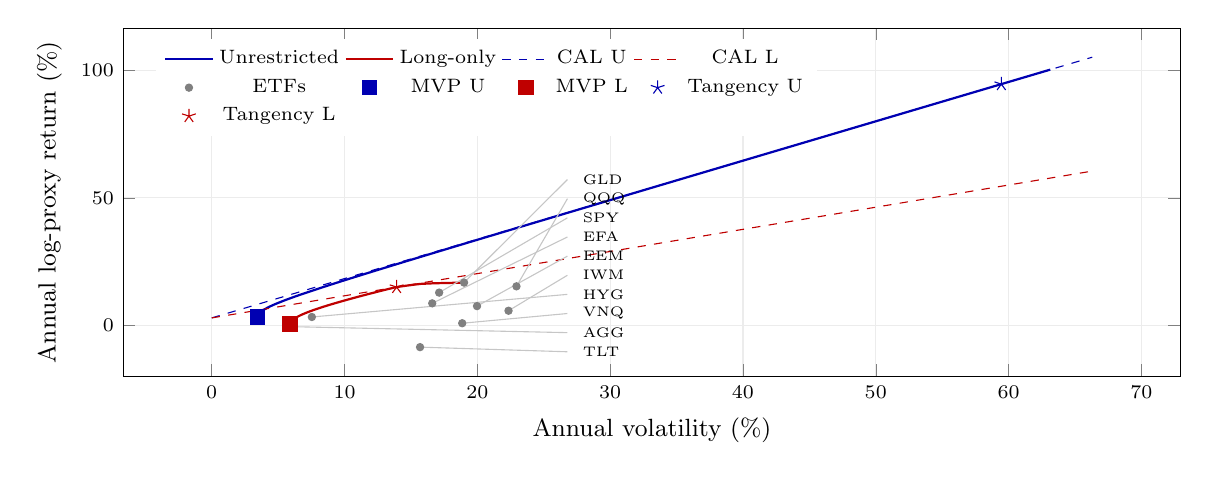
\begin{tikzpicture}\begin{axis}[width=15cm,height=5.1cm,tick label style={font=\scriptsize},label style={font=\small},legend style={font=\scriptsize,draw=none},scaled ticks=false,grid=major,grid style={gray!15},xlabel={Annual volatility (\%)},ylabel={Annual log-proxy return (\%)},legend columns=4,legend pos=north west,height=6cm]
\addplot[blue!70!black,thick] coordinates {(3.445493,3.307582) (3.468234,3.917364) (3.535578,4.527145) (3.645055,5.136926) (3.793017,5.746707) (3.975170,6.356489) (4.187054,6.966270) (4.424400,7.576051) (4.683337,8.185833) (4.960487,8.795614) (5.252966,9.405395) (5.558356,10.015176) (5.874643,10.624958) (6.200161,11.234739) (6.533528,11.844520) (6.873605,12.454301) (7.219441,13.064083) (7.570249,13.673864) (7.925368,14.283645) (8.284243,14.893427) (8.646407,15.503208) (9.011463,16.112989) (9.379073,16.722770) (9.748950,17.332552) (10.120843,17.942333) (10.494540,18.552114) (10.869853,19.161896) (11.246621,19.771677) (11.624703,20.381458) (12.003974,20.991239) (12.384325,21.601021) (12.765659,22.210802) (13.147892,22.820583) (13.530947,23.430365) (13.914755,24.040146) (14.299257,24.649927) (14.684398,25.259708) (15.070128,25.869490) (15.456404,26.479271) (15.843186,27.089052) (16.230438,27.698834) (16.618126,28.308615) (17.006222,28.918396) (17.394697,29.528177) (17.783526,30.137959) (18.172688,30.747740) (18.562161,31.357521) (18.951926,31.967303) (19.341965,32.577084) (19.732263,33.186865) (20.122803,33.796646) (20.513572,34.406428) (20.904558,35.016209) (21.295748,35.625990) (21.687131,36.235772) (22.078698,36.845553) (22.470438,37.455334) (22.862342,38.065115) (23.254403,38.674897) (23.646612,39.284678) (24.038963,39.894459) (24.431448,40.504241) (24.824060,41.114022) (25.216795,41.723803) (25.609647,42.333584) (26.002609,42.943366) (26.395678,43.553147) (26.788848,44.162928) (27.182115,44.772710) (27.575475,45.382491) (27.968924,45.992272) (28.362459,46.602053) (28.756075,47.211835) (29.149770,47.821616) (29.543540,48.431397) (29.937383,49.041178) (30.331295,49.650960) (30.725274,50.260741) (31.119318,50.870522) (31.513423,51.480304) (31.907588,52.090085) (32.301811,52.699866) (32.696089,53.309647) (33.090420,53.919429) (33.484803,54.529210) (33.879236,55.138991) (34.273716,55.748773) (34.668243,56.358554) (35.062815,56.968335) (35.457430,57.578116) (35.852087,58.187898) (36.246784,58.797679) (36.641521,59.407460) (37.036295,60.017242) (37.431107,60.627023) (37.825953,61.236804) (38.220835,61.846585) (38.615750,62.456367) (39.010697,63.066148) (39.405676,63.675929) (39.800685,64.285711) (40.195723,64.895492) (40.590791,65.505273) (40.985886,66.115054) (41.381009,66.724836) (41.776158,67.334617) (42.171332,67.944398) (42.566532,68.554180) (42.961755,69.163961) (43.357002,69.773742) (43.752273,70.383523) (44.147565,70.993305) (44.542879,71.603086) (44.938214,72.212867) (45.333570,72.822649) (45.728945,73.432430) (46.124341,74.042211) (46.519755,74.651992) (46.915188,75.261774) (47.310639,75.871555) (47.706107,76.481336) (48.101593,77.091118) (48.497095,77.700899) (48.892614,78.310680) (49.288149,78.920461) (49.683699,79.530243) (50.079265,80.140024) (50.474846,80.749805) (50.870441,81.359586) (51.266050,81.969368) (51.661673,82.579149) (52.057309,83.188930) (52.452959,83.798712) (52.848622,84.408493) (53.244297,85.018274) (53.639985,85.628055) (54.035685,86.237837) (54.431396,86.847618) (54.827120,87.457399) (55.222854,88.067181) (55.618600,88.676962) (56.014356,89.286743) (56.410124,89.896524) (56.805901,90.506306) (57.201689,91.116087) (57.597486,91.725868) (57.993294,92.335650) (58.389111,92.945431) (58.784937,93.555212) (59.180773,94.164993) (59.576618,94.774775) (59.972471,95.384556) (60.368333,95.994337) (60.764204,96.604119) (61.160082,97.213900) (61.555969,97.823681) (61.951864,98.433462) (62.347767,99.043244) (62.743678,99.653025) (63.139596,100.262806)};
\addlegendentry{Unrestricted}
\addplot[red!75!black,thick] coordinates {(5.902223,0.570347) (5.906822,0.824458) (5.920600,1.078569) (5.943491,1.332679) (5.975392,1.586790) (6.016159,1.840901) (6.065614,2.095012) (6.123545,2.349123) (6.189696,2.603234) (6.262946,2.857345) (6.342589,3.111455) (6.428390,3.365566) (6.520103,3.619677) (6.617484,3.873788) (6.720286,4.127899) (6.828265,4.382010) (6.941178,4.636120) (7.058789,4.890231) (7.180867,5.144342) (7.307188,5.398453) (7.437536,5.652564) (7.571704,5.906675) (7.709491,6.160785) (7.850707,6.414896) (7.995170,6.669007) (8.142708,6.923118) (8.293157,7.177229) (8.446360,7.431340) (8.602171,7.685450) (8.760451,7.939561) (8.921067,8.193672) (9.083897,8.447783) (9.248824,8.701894) (9.415736,8.956005) (9.584531,9.210116) (9.755111,9.464226) (9.927383,9.718337) (10.101262,9.972448) (10.276664,10.226559) (10.453515,10.480670) (10.631742,10.734781) (10.811275,10.988891) (10.992084,11.243002) (11.174548,11.497113) (11.358732,11.751224) (11.544552,12.005335) (11.731932,12.259446) (11.920797,12.513556) (12.111078,12.767667) (12.302710,13.021778) (12.495629,13.275889) (12.689779,13.530000) (12.885102,13.784111) (13.081547,14.038222) (13.279063,14.292332) (13.477604,14.546443) (13.677124,14.800554) (13.896001,15.054665) (14.217797,15.308776) (14.565604,15.562887) (14.932786,15.816997) (15.317950,16.071108) (15.719775,16.325219) (16.769777,16.579330) (19.000707,16.833441)};
\addlegendentry{Long-only}
\addplot[blue!70!black,dashed] coordinates {(0.000000,3.000000) (0.669662,4.031581) (1.339325,5.063162) (2.008987,6.094743) (2.678650,7.126325) (3.348312,8.157906) (4.017974,9.189487) (4.687637,10.221068) (5.357299,11.252649) (6.026961,12.284230) (6.696624,13.315811) (7.366286,14.347392) (8.035949,15.378974) (8.705611,16.410555) (9.375273,17.442136) (10.044936,18.473717) (10.714598,19.505298) (11.384261,20.536879) (12.053923,21.568460) (12.723585,22.600042) (13.393248,23.631623) (14.062910,24.663204) (14.732572,25.694785) (15.402235,26.726366) (16.071897,27.757947) (16.741560,28.789528) (17.411222,29.821110) (18.080884,30.852691) (18.750547,31.884272) (19.420209,32.915853) (20.089871,33.947434) (20.759534,34.979015) (21.429196,36.010596) (22.098859,37.042177) (22.768521,38.073759) (23.438183,39.105340) (24.107846,40.136921) (24.777508,41.168502) (25.447171,42.200083) (26.116833,43.231664) (26.786495,44.263245) (27.456158,45.294827) (28.125820,46.326408) (28.795482,47.357989) (29.465145,48.389570) (30.134807,49.421151) (30.804470,50.452732) (31.474132,51.484313) (32.143794,52.515894) (32.813457,53.547476) (33.483119,54.579057) (34.152782,55.610638) (34.822444,56.642219) (35.492106,57.673800) (36.161769,58.705381) (36.831431,59.736962) (37.501093,60.768544) (38.170756,61.800125) (38.840418,62.831706) (39.510081,63.863287) (40.179743,64.894868) (40.849405,65.926449) (41.519068,66.958030) (42.188730,67.989612) (42.858392,69.021193) (43.528055,70.052774) (44.197717,71.084355) (44.867380,72.115936) (45.537042,73.147517) (46.206704,74.179098) (46.876367,75.210679) (47.546029,76.242261) (48.215692,77.273842) (48.885354,78.305423) (49.555016,79.337004) (50.224679,80.368585) (50.894341,81.400166) (51.564003,82.431747) (52.233666,83.463329) (52.903328,84.494910) (53.572991,85.526491) (54.242653,86.558072) (54.912315,87.589653) (55.581978,88.621234) (56.251640,89.652815) (56.921303,90.684397) (57.590965,91.715978) (58.260627,92.747559) (58.930290,93.779140) (59.599952,94.810721) (60.269614,95.842302) (60.939277,96.873883) (61.608939,97.905464) (62.278602,98.937046) (62.948264,99.968627) (63.617926,101.000208) (64.287589,102.031789) (64.957251,103.063370) (65.626914,104.094951) (66.296576,105.126532)};
\addlegendentry{CAL U}
\addplot[red!75!black,dashed] coordinates {(0.000000,3.000000) (0.669662,3.580955) (1.339325,4.161909) (2.008987,4.742864) (2.678650,5.323819) (3.348312,5.904773) (4.017974,6.485728) (4.687637,7.066682) (5.357299,7.647637) (6.026961,8.228592) (6.696624,8.809546) (7.366286,9.390501) (8.035949,9.971456) (8.705611,10.552410) (9.375273,11.133365) (10.044936,11.714319) (10.714598,12.295274) (11.384261,12.876229) (12.053923,13.457183) (12.723585,14.038138) (13.393248,14.619093) (14.062910,15.200047) (14.732572,15.781002) (15.402235,16.361956) (16.071897,16.942911) (16.741560,17.523866) (17.411222,18.104820) (18.080884,18.685775) (18.750547,19.266730) (19.420209,19.847684) (20.089871,20.428639) (20.759534,21.009593) (21.429196,21.590548) (22.098859,22.171503) (22.768521,22.752457) (23.438183,23.333412) (24.107846,23.914367) (24.777508,24.495321) (25.447171,25.076276) (26.116833,25.657230) (26.786495,26.238185) (27.456158,26.819140) (28.125820,27.400094) (28.795482,27.981049) (29.465145,28.562004) (30.134807,29.142958) (30.804470,29.723913) (31.474132,30.304867) (32.143794,30.885822) (32.813457,31.466777) (33.483119,32.047731) (34.152782,32.628686) (34.822444,33.209641) (35.492106,33.790595) (36.161769,34.371550) (36.831431,34.952504) (37.501093,35.533459) (38.170756,36.114414) (38.840418,36.695368) (39.510081,37.276323) (40.179743,37.857278) (40.849405,38.438232) (41.519068,39.019187) (42.188730,39.600141) (42.858392,40.181096) (43.528055,40.762051) (44.197717,41.343005) (44.867380,41.923960) (45.537042,42.504915) (46.206704,43.085869) (46.876367,43.666824) (47.546029,44.247778) (48.215692,44.828733) (48.885354,45.409688) (49.555016,45.990642) (50.224679,46.571597) (50.894341,47.152552) (51.564003,47.733506) (52.233666,48.314461) (52.903328,48.895415) (53.572991,49.476370) (54.242653,50.057325) (54.912315,50.638279) (55.581978,51.219234) (56.251640,51.800189) (56.921303,52.381143) (57.590965,52.962098) (58.260627,53.543052) (58.930290,54.124007) (59.599952,54.704962) (60.269614,55.285916) (60.939277,55.866871) (61.608939,56.447826) (62.278602,57.028780) (62.948264,57.609735) (63.617926,58.190689) (64.287589,58.771644) (64.957251,59.352599) (65.626914,59.933553) (66.296576,60.514508)};
\addlegendentry{CAL L}
\addplot[only marks,mark=*,mark size=1.3pt,gray] coordinates {(17.124082,12.910442) (22.945709,15.372300) (22.346898,5.812208) (16.602166,8.708111) (19.976124,7.624932) (6.139752,-0.443054) (15.684913,-8.449783) (7.538527,3.360101) (19.000707,16.833441) (18.860998,0.912461)};
\addlegendentry{ETFs}
\draw[gray!45,thin] (axis cs:15.684913,-8.449783) -- (axis description cs:.42,0.07);
\node[font=\fontsize{5.5}{6}\selectfont,anchor=west,xshift=2pt] at (axis description cs:.42,0.07) {TLT};
\draw[gray!45,thin] (axis cs:6.139752,-0.443054) -- (axis description cs:.42,0.125);
\node[font=\fontsize{5.5}{6}\selectfont,anchor=west,xshift=2pt] at (axis description cs:.42,0.125) {AGG};
\draw[gray!45,thin] (axis cs:18.860998,0.912461) -- (axis description cs:.42,0.18);
\node[font=\fontsize{5.5}{6}\selectfont,anchor=west,xshift=2pt] at (axis description cs:.42,0.18) {VNQ};
\draw[gray!45,thin] (axis cs:7.538527,3.360101) -- (axis description cs:.42,0.23500000000000001);
\node[font=\fontsize{5.5}{6}\selectfont,anchor=west,xshift=2pt] at (axis description cs:.42,0.23500000000000001) {HYG};
\draw[gray!45,thin] (axis cs:22.346898,5.812208) -- (axis description cs:.42,0.29000000000000004);
\node[font=\fontsize{5.5}{6}\selectfont,anchor=west,xshift=2pt] at (axis description cs:.42,0.29000000000000004) {IWM};
\draw[gray!45,thin] (axis cs:19.976124,7.624932) -- (axis description cs:.42,0.34500000000000003);
\node[font=\fontsize{5.5}{6}\selectfont,anchor=west,xshift=2pt] at (axis description cs:.42,0.34500000000000003) {EEM};
\draw[gray!45,thin] (axis cs:16.602166,8.708111) -- (axis description cs:.42,0.4);
\node[font=\fontsize{5.5}{6}\selectfont,anchor=west,xshift=2pt] at (axis description cs:.42,0.4) {EFA};
\draw[gray!45,thin] (axis cs:17.124082,12.910442) -- (axis description cs:.42,0.455);
\node[font=\fontsize{5.5}{6}\selectfont,anchor=west,xshift=2pt] at (axis description cs:.42,0.455) {SPY};
\draw[gray!45,thin] (axis cs:22.945709,15.372300) -- (axis description cs:.42,0.51);
\node[font=\fontsize{5.5}{6}\selectfont,anchor=west,xshift=2pt] at (axis description cs:.42,0.51) {QQQ};
\draw[gray!45,thin] (axis cs:19.000707,16.833441) -- (axis description cs:.42,0.565);
\node[font=\fontsize{5.5}{6}\selectfont,anchor=west,xshift=2pt] at (axis description cs:.42,0.565) {GLD};
\addplot[blue!70!black,only marks,mark=square*,mark size=2.6pt] coordinates {(3.445493,3.307582)};
\addlegendentry{MVP U}
\addplot[red!75!black,only marks,mark=square*,mark size=2.6pt] coordinates {(5.902223,0.570347)};
\addlegendentry{MVP L}
\addplot[blue!70!black,only marks,mark=star,mark size=2.6pt] coordinates {(59.455080,94.587553)};
\addlegendentry{Tangency U}
\addplot[red!75!black,only marks,mark=star,mark size=2.6pt] coordinates {(13.922091,15.077882)};
\addlegendentry{Tangency L}
\end{axis}\end{tikzpicture}
\captionof{figure}{Both efficient frontiers, individual ETFs, MVPs, tangencies and CALs on one risk--return chart. }\end{center}
\begin{center}\small
\captionof{table}{Full-sample portfolio risk, return and leverage.}
\begin{tabular}{lrrrr}\toprule
Portfolio & Log mean (\%) & Vol. (\%) & Proxy SR & Gross exposure\\\midrule
MVP U & 3.31 & 3.45 & 0.089 & 2.55 \\
MVP L & 0.57 & 5.90 & -0.412 & 1.00 \\
Tangency U & 94.59 & 59.46 & 1.540 & 16.93 \\
Tangency L & 15.08 & 13.92 & 0.868 & 1.00
\\\bottomrule
\end{tabular}
\end{center}
\begin{center}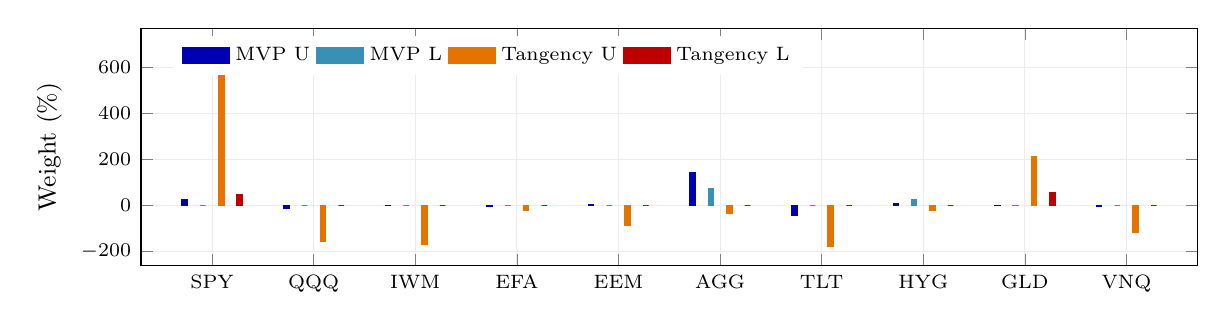
\begin{tikzpicture}\begin{axis}[width=15cm,height=5.1cm,tick label style={font=\scriptsize},label style={font=\small},legend style={font=\scriptsize,draw=none},scaled ticks=false,grid=major,grid style={gray!15},height=4.6cm,xmin=-.7,xmax=9.7,xtick={0,1,2,3,4,5,6,7,8,9},xticklabels={SPY,QQQ,IWM,EFA,EEM,AGG,TLT,HYG,GLD,VNQ},ylabel={Weight (\%)},legend columns=4,legend pos=north west]
\addplot[ybar,area legend,bar shift=0pt,bar width=2pt,fill=blue!70!black,draw=blue!70!black] coordinates {(-0.270000,24.639334) (0.730000,-15.372637) (1.730000,-2.666276) (2.730000,-6.796223) (3.730000,2.835504) (4.730000,143.716478) (5.730000,-44.823074) (6.730000,6.492235) (7.730000,-1.729656) (8.730000,-6.295685)};
\addlegendentry{MVP U}
\addplot[ybar,area legend,bar shift=0pt,bar width=2pt,fill=cyan!70!black,draw=cyan!70!black] coordinates {(-0.090000,0.000000) (0.910000,0.000000) (1.910000,0.000000) (2.910000,0.000000) (3.910000,0.000000) (4.910000,73.469376) (5.910000,0.000000) (6.910000,26.497965) (7.910000,0.032659) (8.910000,0.000000)};
\addlegendentry{MVP L}
\addplot[ybar,area legend,bar shift=0pt,bar width=2pt,fill=orange!90!black,draw=orange!90!black] coordinates {(0.090000,683.310660) (1.090000,-156.303259) (2.090000,-171.745063) (3.090000,-22.446278) (4.090000,-90.375378) (5.090000,-36.676720) (6.090000,-178.097923) (7.090000,-22.629739) (8.090000,212.969992) (9.090000,-118.006292)};
\addlegendentry{Tangency U}
\addplot[ybar,area legend,bar shift=0pt,bar width=2pt,fill=red!75!black,draw=red!75!black] coordinates {(0.270000,44.750435) (1.270000,0.000000) (2.270000,0.000000) (3.270000,0.000000) (4.270000,0.000000) (5.270000,0.000000) (6.270000,0.000000) (7.270000,0.000000) (8.270000,55.249565) (9.270000,0.000000)};
\addlegendentry{Tangency L}
\end{axis}\end{tikzpicture}
\captionof{figure}{Full-sample portfolio allocations. Negative weights denote short positions.}\end{center}
\FullInterpretation

A high fitted Sharpe does not establish a persistent opportunity. Estimated mean differences are amplified by correlated assets and short positions. The MVP does not depend on mean estimates, but still relies on a stable covariance matrix. No-short-sale restrictions can reduce leverage and improve implementability while increasing the attainable variance at a given target return.
\heading{4. Out-of-sample robustness}
Estimate weights only on the first three years, ending \SplitDate{}, then hold those target weights fixed throughout the remaining two years. The split produces \InDays{} in-sample and \OutDays{} out-of-sample returns with no shared return dates. Daily rebalancing uses exact portfolio simple returns $R_{p,t}=w^\top[\exp(\ell_t)-\mathbf1]$ and wealth $V_t=\prod_{s\le t}(1+R_{p,s})$, beginning at $V_0=1$. Any daily return at or below $-1$ triggers insolvency handling rather than an invalid logarithm.

The realized Sharpe uses daily simple excess returns over $r_{f,d}=(1.03)^{1/252}-1$:
\[
 S=\sqrt{252}\,\frac{\overline{R_p-r_{f,d}}}{s(R_p-r_{f,d})}.
\]
Reported geometric growth is $V_T^{252/T}-1$. It is not the same statistic as the log-moment model's linear predicted return.
\ISDiagnostic
\newpage
\begin{center}\small
\captionof{table}{In-sample and out-of-sample performance.}
\begin{tabular}{lrrrrr}\toprule
Strategy & IS SR & OOS SR & Growth (\%) & Vol. (\%) & Max DD (\%)\\\midrule
MVP U & -0.263 & 0.154 & 3.38 & 2.61 & -1.73 \\
MVP L & -0.437 & -0.027 & 2.78 & 4.30 & -4.15 \\
Tangency L & 0.917 & 1.052 & 23.19 & 18.68 & -17.50 \\
Equal weight & 0.153 & 0.796 & 12.21 & 11.60 & -10.54 \\
Bounded diagnostic & 1.797 & 1.060 & 41.07 & 35.73 & -46.32
\\\bottomrule
\end{tabular}
\end{center}
\begin{center}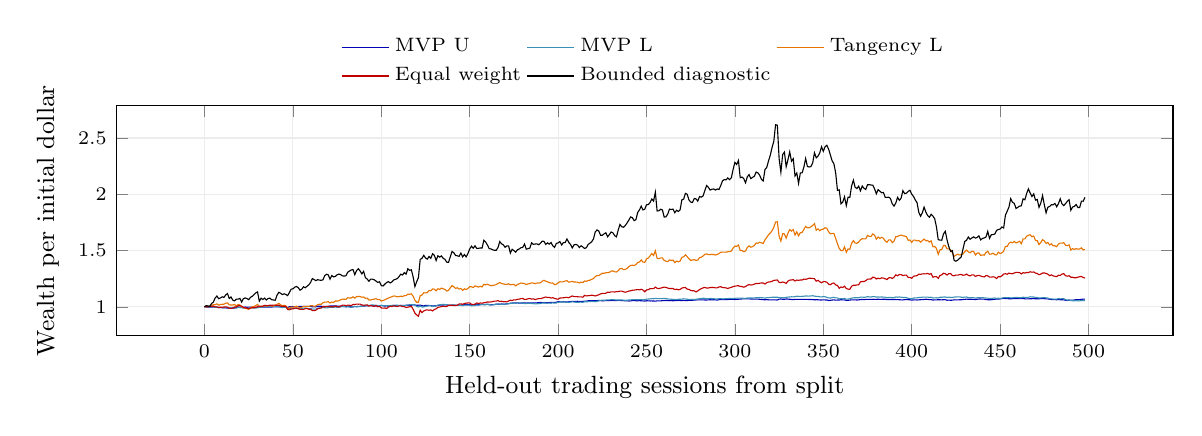
\begin{tikzpicture}\begin{axis}[width=15cm,height=5.1cm,tick label style={font=\scriptsize},label style={font=\small},legend style={font=\scriptsize,draw=none},scaled ticks=false,grid=major,grid style={gray!15},height=4.5cm,xlabel={Held-out trading sessions from split},ylabel={Wealth per initial dollar},legend columns=3,legend style={at={(.5,1.04)},anchor=south,font=\scriptsize,draw=none},legend cell align=left]
\addplot[blue!70!black,thin] coordinates {(0.000000,1.000000) (1.000000,0.998280) (2.000000,0.998187) (3.000000,0.998305) (4.000000,0.998371) (5.000000,0.998026) (6.000000,0.997156) (7.000000,0.996546) (8.000000,0.994626) (9.000000,0.992787) (10.000000,0.992027) (11.000000,0.990758) (12.000000,0.990822) (13.000000,0.988019) (14.000000,0.988113) (15.000000,0.989227) (16.000000,0.987606) (17.000000,0.988361) (18.000000,0.993791) (19.000000,0.997223) (20.000000,0.994149) (21.000000,0.994019) (22.000000,0.993872) (23.000000,0.998531) (24.000000,0.995285) (25.000000,0.997742) (26.000000,0.997042) (27.000000,0.995942) (28.000000,0.996087) (29.000000,0.995325) (30.000000,0.995024) (31.000000,0.996908) (32.000000,0.996999) (33.000000,0.997541) (34.000000,0.998015) (35.000000,0.997094) (36.000000,0.997787) (37.000000,0.997499) (38.000000,0.997507) (39.000000,0.999958) (40.000000,1.000085) (41.000000,1.000805) (42.000000,1.000045) (43.000000,1.000491) (44.000000,0.999057) (45.000000,0.997829) (46.000000,0.997047) (47.000000,0.994599) (48.000000,0.999914) (49.000000,1.001969) (50.000000,1.001122) (51.000000,1.000903) (52.000000,1.001195) (53.000000,1.002280) (54.000000,1.004366) (55.000000,1.004289) (56.000000,1.003216) (57.000000,1.002952) (58.000000,1.003523) (59.000000,1.003610) (60.000000,1.004759) (61.000000,1.000019) (62.000000,0.999134) (63.000000,1.000015) (64.000000,1.004986) (65.000000,1.005091) (66.000000,1.004461) (67.000000,1.003487) (68.000000,1.003167) (69.000000,1.004321) (70.000000,1.004328) (71.000000,1.007130) (72.000000,1.007892) (73.000000,1.008126) (74.000000,1.007537) (75.000000,1.006575) (76.000000,1.004540) (77.000000,1.004894) (78.000000,1.003387) (79.000000,1.001911) (80.000000,1.000736) (81.000000,1.001702) (82.000000,1.001242) (83.000000,0.999237) (84.000000,0.999226) (85.000000,1.002752) (86.000000,1.001166) (87.000000,1.004173) (88.000000,1.004149) (89.000000,1.005503) (90.000000,1.006582) (91.000000,1.007853) (92.000000,1.007922) (93.000000,1.009715) (94.000000,1.011284) (95.000000,1.009468) (96.000000,1.009410) (97.000000,1.006992) (98.000000,1.009690) (99.000000,1.008503) (100.000000,1.012395) (101.000000,1.009279) (102.000000,1.006811) (103.000000,1.008142) (104.000000,1.006628) (105.000000,1.005584) (106.000000,1.006415) (107.000000,1.008715) (108.000000,1.009543) (109.000000,1.011468) (110.000000,1.010431) (111.000000,1.011783) (112.000000,1.011519) (113.000000,1.012133) (114.000000,1.013401) (115.000000,1.013348) (116.000000,1.014448) (117.000000,1.012661) (118.000000,1.018195) (119.000000,1.016109) (120.000000,1.012981) (121.000000,1.014330) (122.000000,1.014235) (123.000000,1.011721) (124.000000,1.007162) (125.000000,1.012403) (126.000000,1.011595) (127.000000,1.011395) (128.000000,1.010400) (129.000000,1.007792) (130.000000,1.008667) (131.000000,1.009234) (132.000000,1.012279) (133.000000,1.014724) (134.000000,1.014576) (135.000000,1.014953) (136.000000,1.017704) (137.000000,1.016319) (138.000000,1.013950) (139.000000,1.012590) (140.000000,1.013607) (141.000000,1.014737) (142.000000,1.013126) (143.000000,1.012861) (144.000000,1.015243) (145.000000,1.015500) (146.000000,1.015938) (147.000000,1.018699) (148.000000,1.018652) (149.000000,1.018550) (150.000000,1.018078) (151.000000,1.016036) (152.000000,1.018428) (153.000000,1.018684) (154.000000,1.018691) (155.000000,1.018027) (156.000000,1.019055) (157.000000,1.021732) (158.000000,1.020505) (159.000000,1.021450) (160.000000,1.022252) (161.000000,1.018483) (162.000000,1.017551) (163.000000,1.018916) (164.000000,1.019873) (165.000000,1.024007) (166.000000,1.023562) (167.000000,1.022389) (168.000000,1.024782) (169.000000,1.023916) (170.000000,1.023882) (171.000000,1.026796) (172.000000,1.027746) (173.000000,1.031539) (174.000000,1.033054) (175.000000,1.034798) (176.000000,1.033880) (177.000000,1.034928) (178.000000,1.032908) (179.000000,1.033371) (180.000000,1.034273) (181.000000,1.033507) (182.000000,1.033245) (183.000000,1.034219) (184.000000,1.034052) (185.000000,1.033899) (186.000000,1.034182) (187.000000,1.034308) (188.000000,1.035452) (189.000000,1.036538) (190.000000,1.038640) (191.000000,1.037355) (192.000000,1.036192) (193.000000,1.035560) (194.000000,1.036294) (195.000000,1.036997) (196.000000,1.039915) (197.000000,1.038740) (198.000000,1.038292) (199.000000,1.040365) (200.000000,1.045412) (201.000000,1.044522) (202.000000,1.042874) (203.000000,1.045397) (204.000000,1.043142) (205.000000,1.042962) (206.000000,1.044811) (207.000000,1.046655) (208.000000,1.048212) (209.000000,1.047977) (210.000000,1.048254) (211.000000,1.048930) (212.000000,1.048657) (213.000000,1.047929) (214.000000,1.046986) (215.000000,1.051015) (216.000000,1.050777) (217.000000,1.053248) (218.000000,1.054990) (219.000000,1.053446) (220.000000,1.054603) (221.000000,1.054535) (222.000000,1.055003) (223.000000,1.057197) (224.000000,1.054781) (225.000000,1.053202) (226.000000,1.053895) (227.000000,1.055565) (228.000000,1.054875) (229.000000,1.055368) (230.000000,1.056401) (231.000000,1.056721) (232.000000,1.055987) (233.000000,1.055282) (234.000000,1.056955) (235.000000,1.056269) (236.000000,1.054620) (237.000000,1.054805) (238.000000,1.052540) (239.000000,1.053146) (240.000000,1.051644) (241.000000,1.052659) (242.000000,1.055062) (243.000000,1.055499) (244.000000,1.054110) (245.000000,1.054074) (246.000000,1.054535) (247.000000,1.053649) (248.000000,1.052954) (249.000000,1.050848) (250.000000,1.053545) (251.000000,1.053187) (252.000000,1.051960) (253.000000,1.052171) (254.000000,1.051502) (255.000000,1.050462) (256.000000,1.052733) (257.000000,1.052505) (258.000000,1.052898) (259.000000,1.054632) (260.000000,1.055219) (261.000000,1.056306) (262.000000,1.056113) (263.000000,1.054196) (264.000000,1.054747) (265.000000,1.054016) (266.000000,1.054831) (267.000000,1.054652) (268.000000,1.057061) (269.000000,1.056272) (270.000000,1.055164) (271.000000,1.057289) (272.000000,1.055645) (273.000000,1.055738) (274.000000,1.057123) (275.000000,1.057032) (276.000000,1.057986) (277.000000,1.059711) (278.000000,1.060718) (279.000000,1.061618) (280.000000,1.060994) (281.000000,1.062082) (282.000000,1.061512) (283.000000,1.060638) (284.000000,1.060331) (285.000000,1.061587) (286.000000,1.062903) (287.000000,1.061868) (288.000000,1.062772) (289.000000,1.062088) (290.000000,1.059738) (291.000000,1.063164) (292.000000,1.063725) (293.000000,1.063773) (294.000000,1.064735) (295.000000,1.064659) (296.000000,1.064601) (297.000000,1.066233) (298.000000,1.066055) (299.000000,1.065976) (300.000000,1.065159) (301.000000,1.065899) (302.000000,1.067502) (303.000000,1.069288) (304.000000,1.069884) (305.000000,1.070439) (306.000000,1.071648) (307.000000,1.070869) (308.000000,1.070620) (309.000000,1.069384) (310.000000,1.068822) (311.000000,1.068165) (312.000000,1.068312) (313.000000,1.068300) (314.000000,1.066904) (315.000000,1.064924) (316.000000,1.063635) (317.000000,1.062534) (318.000000,1.063816) (319.000000,1.062259) (320.000000,1.061368) (321.000000,1.061478) (322.000000,1.061392) (323.000000,1.061772) (324.000000,1.060089) (325.000000,1.067981) (326.000000,1.069673) (327.000000,1.066686) (328.000000,1.066878) (329.000000,1.069898) (330.000000,1.068586) (331.000000,1.066895) (332.000000,1.065211) (333.000000,1.063803) (334.000000,1.065609) (335.000000,1.065468) (336.000000,1.065833) (337.000000,1.065765) (338.000000,1.065636) (339.000000,1.066573) (340.000000,1.066052) (341.000000,1.065994) (342.000000,1.064998) (343.000000,1.064731) (344.000000,1.063743) (345.000000,1.062052) (346.000000,1.063395) (347.000000,1.062380) (348.000000,1.060938) (349.000000,1.060727) (350.000000,1.061909) (351.000000,1.060928) (352.000000,1.060924) (353.000000,1.056006) (354.000000,1.057745) (355.000000,1.060261) (356.000000,1.061742) (357.000000,1.059275) (358.000000,1.060057) (359.000000,1.060039) (360.000000,1.063273) (361.000000,1.061541) (362.000000,1.061188) (363.000000,1.057250) (364.000000,1.058158) (365.000000,1.059625) (366.000000,1.062067) (367.000000,1.061573) (368.000000,1.061901) (369.000000,1.060140) (370.000000,1.061951) (371.000000,1.063911) (372.000000,1.065665) (373.000000,1.063538) (374.000000,1.065888) (375.000000,1.066132) (376.000000,1.066022) (377.000000,1.066316) (378.000000,1.066704) (379.000000,1.066534) (380.000000,1.065922) (381.000000,1.067814) (382.000000,1.065579) (383.000000,1.066190) (384.000000,1.067624) (385.000000,1.066972) (386.000000,1.064243) (387.000000,1.064972) (388.000000,1.064843) (389.000000,1.065249) (390.000000,1.064422) (391.000000,1.064468) (392.000000,1.064018) (393.000000,1.062956) (394.000000,1.061747) (395.000000,1.060845) (396.000000,1.063650) (397.000000,1.064740) (398.000000,1.063376) (399.000000,1.062587) (400.000000,1.059321) (401.000000,1.061191) (402.000000,1.061264) (403.000000,1.060791) (404.000000,1.061709) (405.000000,1.063124) (406.000000,1.063999) (407.000000,1.065272) (408.000000,1.067345) (409.000000,1.065726) (410.000000,1.063388) (411.000000,1.063683) (412.000000,1.059993) (413.000000,1.061340) (414.000000,1.061768) (415.000000,1.063113) (416.000000,1.062639) (417.000000,1.061529) (418.000000,1.063161) (419.000000,1.063180) (420.000000,1.058087) (421.000000,1.059720) (422.000000,1.057824) (423.000000,1.059132) (424.000000,1.062312) (425.000000,1.061369) (426.000000,1.061266) (427.000000,1.062196) (428.000000,1.062506) (429.000000,1.064746) (430.000000,1.066145) (431.000000,1.067936) (432.000000,1.067254) (433.000000,1.066930) (434.000000,1.066944) (435.000000,1.065989) (436.000000,1.064038) (437.000000,1.066963) (438.000000,1.069156) (439.000000,1.069246) (440.000000,1.067823) (441.000000,1.068135) (442.000000,1.064039) (443.000000,1.063044) (444.000000,1.062420) (445.000000,1.063293) (446.000000,1.064444) (447.000000,1.067350) (448.000000,1.068087) (449.000000,1.068113) (450.000000,1.070371) (451.000000,1.073055) (452.000000,1.074790) (453.000000,1.073835) (454.000000,1.072641) (455.000000,1.071724) (456.000000,1.071289) (457.000000,1.072319) (458.000000,1.073073) (459.000000,1.073992) (460.000000,1.072779) (461.000000,1.072887) (462.000000,1.074630) (463.000000,1.073133) (464.000000,1.071131) (465.000000,1.069944) (466.000000,1.070006) (467.000000,1.071928) (468.000000,1.071938) (469.000000,1.073003) (470.000000,1.071308) (471.000000,1.072041) (472.000000,1.071388) (473.000000,1.072460) (474.000000,1.072328) (475.000000,1.072325) (476.000000,1.070556) (477.000000,1.070220) (478.000000,1.066852) (479.000000,1.065015) (480.000000,1.063748) (481.000000,1.064580) (482.000000,1.062611) (483.000000,1.065148) (484.000000,1.062865) (485.000000,1.062845) (486.000000,1.061923) (487.000000,1.057621) (488.000000,1.056217) (489.000000,1.060099) (490.000000,1.058131) (491.000000,1.058809) (492.000000,1.060603) (493.000000,1.063715) (494.000000,1.062119) (495.000000,1.063787) (496.000000,1.066188) (497.000000,1.068266) (498.000000,1.067870)};
\addlegendentry{MVP U}
\addplot[cyan!70!black,thin] coordinates {(0.000000,1.000000) (1.000000,0.999356) (2.000000,1.002292) (3.000000,1.003831) (4.000000,0.999934) (5.000000,1.001307) (6.000000,0.995158) (7.000000,0.995277) (8.000000,0.992392) (9.000000,0.994634) (10.000000,0.992946) (11.000000,0.992291) (12.000000,0.993437) (13.000000,0.992380) (14.000000,0.991210) (15.000000,0.988149) (16.000000,0.991940) (17.000000,0.994428) (18.000000,0.988073) (19.000000,0.995179) (20.000000,0.996494) (21.000000,0.993930) (22.000000,0.988387) (23.000000,0.987993) (24.000000,0.987137) (25.000000,0.987142) (26.000000,0.988777) (27.000000,0.990385) (28.000000,0.989703) (29.000000,0.989597) (30.000000,0.990405) (31.000000,0.997194) (32.000000,0.995673) (33.000000,0.998437) (34.000000,1.002069) (35.000000,1.001886) (36.000000,1.000496) (37.000000,1.003548) (38.000000,1.003368) (39.000000,1.005857) (40.000000,1.003758) (41.000000,1.003178) (42.000000,1.001739) (43.000000,0.997679) (44.000000,0.993928) (45.000000,0.995044) (46.000000,0.994479) (47.000000,0.985952) (48.000000,0.983873) (49.000000,0.987471) (50.000000,0.984520) (51.000000,0.986103) (52.000000,0.987323) (53.000000,0.984862) (54.000000,0.987950) (55.000000,0.987136) (56.000000,0.988052) (57.000000,0.987463) (58.000000,0.987056) (59.000000,0.983841) (60.000000,0.985058) (61.000000,0.979937) (62.000000,0.978898) (63.000000,0.979596) (64.000000,0.988100) (65.000000,0.990126) (66.000000,0.990228) (67.000000,0.993712) (68.000000,0.991779) (69.000000,0.990788) (70.000000,0.992461) (71.000000,0.996415) (72.000000,0.996371) (73.000000,0.995679) (74.000000,0.997650) (75.000000,0.995658) (76.000000,0.996192) (77.000000,0.998619) (78.000000,1.003351) (79.000000,1.002214) (80.000000,0.999184) (81.000000,1.000353) (82.000000,0.998449) (83.000000,0.994102) (84.000000,0.999854) (85.000000,1.002559) (86.000000,0.999811) (87.000000,1.001062) (88.000000,1.002432) (89.000000,1.005248) (90.000000,1.006873) (91.000000,1.011802) (92.000000,1.013440) (93.000000,1.011356) (94.000000,1.015101) (95.000000,1.016592) (96.000000,1.014909) (97.000000,1.012630) (98.000000,1.010871) (99.000000,1.010338) (100.000000,1.012795) (101.000000,1.009679) (102.000000,1.007825) (103.000000,1.009385) (104.000000,1.008950) (105.000000,1.010724) (106.000000,1.011387) (107.000000,1.015175) (108.000000,1.015248) (109.000000,1.013750) (110.000000,1.011343) (111.000000,1.012028) (112.000000,1.009237) (113.000000,1.008818) (114.000000,1.012932) (115.000000,1.015011) (116.000000,1.018320) (117.000000,1.017967) (118.000000,1.019027) (119.000000,1.015665) (120.000000,1.003289) (121.000000,0.998419) (122.000000,1.007192) (123.000000,0.998224) (124.000000,0.998772) (125.000000,1.004170) (126.000000,1.006433) (127.000000,1.009573) (128.000000,1.008816) (129.000000,1.003745) (130.000000,1.005711) (131.000000,1.008118) (132.000000,1.014700) (133.000000,1.017409) (134.000000,1.020004) (135.000000,1.022218) (136.000000,1.020184) (137.000000,1.017823) (138.000000,1.014969) (139.000000,1.014376) (140.000000,1.016789) (141.000000,1.017694) (142.000000,1.013131) (143.000000,1.014283) (144.000000,1.013251) (145.000000,1.012967) (146.000000,1.009487) (147.000000,1.014623) (148.000000,1.015023) (149.000000,1.015025) (150.000000,1.014055) (151.000000,1.007757) (152.000000,1.010146) (153.000000,1.011781) (154.000000,1.016096) (155.000000,1.014458) (156.000000,1.017790) (157.000000,1.019617) (158.000000,1.018291) (159.000000,1.017935) (160.000000,1.023170) (161.000000,1.020635) (162.000000,1.016338) (163.000000,1.017572) (164.000000,1.019872) (165.000000,1.022589) (166.000000,1.026009) (167.000000,1.022828) (168.000000,1.021399) (169.000000,1.023448) (170.000000,1.024187) (171.000000,1.025533) (172.000000,1.027654) (173.000000,1.031171) (174.000000,1.031123) (175.000000,1.033896) (176.000000,1.031076) (177.000000,1.035411) (178.000000,1.034661) (179.000000,1.034298) (180.000000,1.032702) (181.000000,1.029117) (182.000000,1.028267) (183.000000,1.032222) (184.000000,1.031842) (185.000000,1.028552) (186.000000,1.028551) (187.000000,1.025536) (188.000000,1.027380) (189.000000,1.027897) (190.000000,1.029677) (191.000000,1.032564) (192.000000,1.034706) (193.000000,1.032812) (194.000000,1.031867) (195.000000,1.033009) (196.000000,1.031655) (197.000000,1.036068) (198.000000,1.032881) (199.000000,1.033550) (200.000000,1.040798) (201.000000,1.042404) (202.000000,1.042572) (203.000000,1.042451) (204.000000,1.041874) (205.000000,1.040382) (206.000000,1.040539) (207.000000,1.041093) (208.000000,1.044692) (209.000000,1.041639) (210.000000,1.040636) (211.000000,1.039595) (212.000000,1.040850) (213.000000,1.041503) (214.000000,1.039156) (215.000000,1.045731) (216.000000,1.043996) (217.000000,1.045621) (218.000000,1.046704) (219.000000,1.047991) (220.000000,1.046770) (221.000000,1.045055) (222.000000,1.048772) (223.000000,1.052435) (224.000000,1.056735) (225.000000,1.059815) (226.000000,1.057946) (227.000000,1.059851) (228.000000,1.061982) (229.000000,1.061091) (230.000000,1.063418) (231.000000,1.063675) (232.000000,1.061837) (233.000000,1.059980) (234.000000,1.060334) (235.000000,1.060042) (236.000000,1.061269) (237.000000,1.059177) (238.000000,1.057493) (239.000000,1.058639) (240.000000,1.061052) (241.000000,1.061146) (242.000000,1.063710) (243.000000,1.064446) (244.000000,1.063550) (245.000000,1.062383) (246.000000,1.063583) (247.000000,1.063828) (248.000000,1.061650) (249.000000,1.063639) (250.000000,1.067430) (251.000000,1.069098) (252.000000,1.070096) (253.000000,1.072849) (254.000000,1.071807) (255.000000,1.074709) (256.000000,1.073339) (257.000000,1.073030) (258.000000,1.072268) (259.000000,1.073644) (260.000000,1.074084) (261.000000,1.074142) (262.000000,1.069529) (263.000000,1.068048) (264.000000,1.067403) (265.000000,1.065799) (266.000000,1.065629) (267.000000,1.064060) (268.000000,1.067039) (269.000000,1.067061) (270.000000,1.068365) (271.000000,1.071151) (272.000000,1.070817) (273.000000,1.067166) (274.000000,1.065770) (275.000000,1.065172) (276.000000,1.065874) (277.000000,1.066008) (278.000000,1.066730) (279.000000,1.069381) (280.000000,1.072116) (281.000000,1.074212) (282.000000,1.075994) (283.000000,1.075330) (284.000000,1.071537) (285.000000,1.072841) (286.000000,1.074556) (287.000000,1.072801) (288.000000,1.071914) (289.000000,1.069967) (290.000000,1.069113) (291.000000,1.072659) (292.000000,1.073054) (293.000000,1.070192) (294.000000,1.071120) (295.000000,1.072762) (296.000000,1.072421) (297.000000,1.075098) (298.000000,1.073899) (299.000000,1.074441) (300.000000,1.075012) (301.000000,1.077129) (302.000000,1.077546) (303.000000,1.077398) (304.000000,1.077348) (305.000000,1.074971) (306.000000,1.075170) (307.000000,1.078106) (308.000000,1.078348) (309.000000,1.078791) (310.000000,1.077650) (311.000000,1.079844) (312.000000,1.080161) (313.000000,1.080804) (314.000000,1.082336) (315.000000,1.081149) (316.000000,1.079747) (317.000000,1.077026) (318.000000,1.080913) (319.000000,1.081807) (320.000000,1.082851) (321.000000,1.084605) (322.000000,1.084819) (323.000000,1.085239) (324.000000,1.085250) (325.000000,1.082352) (326.000000,1.080468) (327.000000,1.082193) (328.000000,1.081303) (329.000000,1.083807) (330.000000,1.086130) (331.000000,1.087443) (332.000000,1.089329) (333.000000,1.087841) (334.000000,1.090376) (335.000000,1.093887) (336.000000,1.092957) (337.000000,1.092763) (338.000000,1.093073) (339.000000,1.094107) (340.000000,1.096045) (341.000000,1.095515) (342.000000,1.095431) (343.000000,1.096712) (344.000000,1.098326) (345.000000,1.095115) (346.000000,1.092152) (347.000000,1.092928) (348.000000,1.089118) (349.000000,1.087406) (350.000000,1.091505) (351.000000,1.088760) (352.000000,1.084466) (353.000000,1.079187) (354.000000,1.077723) (355.000000,1.081815) (356.000000,1.084474) (357.000000,1.078827) (358.000000,1.079357) (359.000000,1.069345) (360.000000,1.073465) (361.000000,1.070389) (362.000000,1.074902) (363.000000,1.067612) (364.000000,1.067874) (365.000000,1.072163) (366.000000,1.077504) (367.000000,1.079150) (368.000000,1.080989) (369.000000,1.079863) (370.000000,1.081201) (371.000000,1.085251) (372.000000,1.086201) (373.000000,1.083861) (374.000000,1.086322) (375.000000,1.089908) (376.000000,1.088180) (377.000000,1.086712) (378.000000,1.091129) (379.000000,1.090555) (380.000000,1.086009) (381.000000,1.088030) (382.000000,1.085954) (383.000000,1.087722) (384.000000,1.086345) (385.000000,1.085115) (386.000000,1.080384) (387.000000,1.082811) (388.000000,1.084157) (389.000000,1.080286) (390.000000,1.082498) (391.000000,1.087725) (392.000000,1.084823) (393.000000,1.087812) (394.000000,1.085247) (395.000000,1.082204) (396.000000,1.082643) (397.000000,1.082029) (398.000000,1.074889) (399.000000,1.075101) (400.000000,1.070877) (401.000000,1.077749) (402.000000,1.078892) (403.000000,1.079525) (404.000000,1.082898) (405.000000,1.083050) (406.000000,1.085305) (407.000000,1.086322) (408.000000,1.085501) (409.000000,1.086041) (410.000000,1.083300) (411.000000,1.085211) (412.000000,1.078518) (413.000000,1.079032) (414.000000,1.080483) (415.000000,1.078290) (416.000000,1.085534) (417.000000,1.084593) (418.000000,1.086572) (419.000000,1.087504) (420.000000,1.083012) (421.000000,1.086349) (422.000000,1.083767) (423.000000,1.083313) (424.000000,1.086411) (425.000000,1.087335) (426.000000,1.088168) (427.000000,1.088590) (428.000000,1.085333) (429.000000,1.084032) (430.000000,1.085772) (431.000000,1.087143) (432.000000,1.082551) (433.000000,1.080679) (434.000000,1.082436) (435.000000,1.081415) (436.000000,1.076815) (437.000000,1.080190) (438.000000,1.081735) (439.000000,1.080930) (440.000000,1.081243) (441.000000,1.079219) (442.000000,1.078117) (443.000000,1.076688) (444.000000,1.073262) (445.000000,1.074154) (446.000000,1.076416) (447.000000,1.078243) (448.000000,1.074629) (449.000000,1.076607) (450.000000,1.074200) (451.000000,1.076762) (452.000000,1.081162) (453.000000,1.082601) (454.000000,1.080012) (455.000000,1.082556) (456.000000,1.079394) (457.000000,1.080072) (458.000000,1.081664) (459.000000,1.083982) (460.000000,1.082158) (461.000000,1.080289) (462.000000,1.080223) (463.000000,1.085819) (464.000000,1.082765) (465.000000,1.082325) (466.000000,1.084377) (467.000000,1.089086) (468.000000,1.087323) (469.000000,1.087115) (470.000000,1.082938) (471.000000,1.082425) (472.000000,1.078263) (473.000000,1.079337) (474.000000,1.081093) (475.000000,1.081265) (476.000000,1.079843) (477.000000,1.077799) (478.000000,1.070824) (479.000000,1.070428) (480.000000,1.068874) (481.000000,1.068170) (482.000000,1.067779) (483.000000,1.073609) (484.000000,1.070148) (485.000000,1.072684) (486.000000,1.073135) (487.000000,1.063776) (488.000000,1.059165) (489.000000,1.060703) (490.000000,1.054676) (491.000000,1.054108) (492.000000,1.052963) (493.000000,1.055000) (494.000000,1.053498) (495.000000,1.052753) (496.000000,1.055687) (497.000000,1.054464) (498.000000,1.055749)};
\addlegendentry{MVP L}
\addplot[orange!90!black,thin] coordinates {(0.000000,1.000000) (1.000000,1.001260) (2.000000,1.001418) (3.000000,1.006233) (4.000000,1.010509) (5.000000,1.019223) (6.000000,1.018587) (7.000000,1.026178) (8.000000,1.014693) (9.000000,1.020846) (10.000000,1.022223) (11.000000,1.023183) (12.000000,1.031534) (13.000000,1.034621) (14.000000,1.017337) (15.000000,1.015658) (16.000000,1.016035) (17.000000,1.021270) (18.000000,1.006861) (19.000000,1.020573) (20.000000,1.017002) (21.000000,1.000449) (22.000000,0.993442) (23.000000,0.986520) (24.000000,0.982835) (25.000000,0.977898) (26.000000,0.992199) (27.000000,0.999538) (28.000000,1.003608) (29.000000,1.011100) (30.000000,1.021218) (31.000000,1.001017) (32.000000,1.003926) (33.000000,1.004604) (34.000000,1.012554) (35.000000,1.006836) (36.000000,1.008403) (37.000000,1.012405) (38.000000,1.006632) (39.000000,1.007457) (40.000000,1.012978) (41.000000,1.021457) (42.000000,1.030653) (43.000000,1.018427) (44.000000,1.009681) (45.000000,1.012671) (46.000000,1.008700) (47.000000,0.986193) (48.000000,0.987092) (49.000000,0.997850) (50.000000,0.996296) (51.000000,1.000958) (52.000000,1.005745) (53.000000,0.997752) (54.000000,0.992152) (55.000000,0.995452) (56.000000,1.004272) (57.000000,1.002401) (58.000000,1.003231) (59.000000,1.003876) (60.000000,1.008072) (61.000000,1.010335) (62.000000,1.003704) (63.000000,1.007828) (64.000000,1.018553) (65.000000,1.022941) (66.000000,1.022137) (67.000000,1.036059) (68.000000,1.041528) (69.000000,1.042163) (70.000000,1.045838) (71.000000,1.033804) (72.000000,1.042734) (73.000000,1.038532) (74.000000,1.051269) (75.000000,1.051086) (76.000000,1.052960) (77.000000,1.062356) (78.000000,1.068278) (79.000000,1.067375) (80.000000,1.065840) (81.000000,1.080707) (82.000000,1.078165) (83.000000,1.077939) (84.000000,1.088791) (85.000000,1.077353) (86.000000,1.090870) (87.000000,1.092054) (88.000000,1.091113) (89.000000,1.084905) (90.000000,1.087606) (91.000000,1.075894) (92.000000,1.077213) (93.000000,1.060567) (94.000000,1.060755) (95.000000,1.065143) (96.000000,1.067963) (97.000000,1.072913) (98.000000,1.063456) (99.000000,1.065604) (100.000000,1.050660) (101.000000,1.056779) (102.000000,1.061671) (103.000000,1.070800) (104.000000,1.077618) (105.000000,1.084181) (106.000000,1.089655) (107.000000,1.096309) (108.000000,1.094384) (109.000000,1.088276) (110.000000,1.090600) (111.000000,1.094757) (112.000000,1.090269) (113.000000,1.099726) (114.000000,1.098952) (115.000000,1.112259) (116.000000,1.111633) (117.000000,1.115314) (118.000000,1.094371) (119.000000,1.057438) (120.000000,1.040857) (121.000000,1.040051) (122.000000,1.099368) (123.000000,1.104116) (124.000000,1.124785) (125.000000,1.123473) (126.000000,1.126692) (127.000000,1.145177) (128.000000,1.142111) (129.000000,1.159025) (130.000000,1.156303) (131.000000,1.142023) (132.000000,1.160831) (133.000000,1.154425) (134.000000,1.166152) (135.000000,1.160305) (136.000000,1.154317) (137.000000,1.139813) (138.000000,1.146203) (139.000000,1.168416) (140.000000,1.188636) (141.000000,1.177537) (142.000000,1.163596) (143.000000,1.169114) (144.000000,1.157248) (145.000000,1.162976) (146.000000,1.146155) (147.000000,1.160711) (148.000000,1.152981) (149.000000,1.163828) (150.000000,1.177963) (151.000000,1.178247) (152.000000,1.171019) (153.000000,1.186759) (154.000000,1.179839) (155.000000,1.175943) (156.000000,1.182225) (157.000000,1.176350) (158.000000,1.200359) (159.000000,1.194878) (160.000000,1.200213) (161.000000,1.194229) (162.000000,1.186540) (163.000000,1.190804) (164.000000,1.193040) (165.000000,1.196592) (166.000000,1.208477) (167.000000,1.215664) (168.000000,1.206844) (169.000000,1.204243) (170.000000,1.199614) (171.000000,1.198430) (172.000000,1.204507) (173.000000,1.195071) (174.000000,1.197828) (175.000000,1.199654) (176.000000,1.186073) (177.000000,1.197771) (178.000000,1.205195) (179.000000,1.211504) (180.000000,1.208486) (181.000000,1.206472) (182.000000,1.197389) (183.000000,1.203281) (184.000000,1.206170) (185.000000,1.213090) (186.000000,1.210644) (187.000000,1.205571) (188.000000,1.211001) (189.000000,1.211327) (190.000000,1.213288) (191.000000,1.227120) (192.000000,1.235382) (193.000000,1.227672) (194.000000,1.222493) (195.000000,1.216038) (196.000000,1.210395) (197.000000,1.211803) (198.000000,1.196588) (199.000000,1.200874) (200.000000,1.212272) (201.000000,1.222680) (202.000000,1.221547) (203.000000,1.222476) (204.000000,1.229450) (205.000000,1.232081) (206.000000,1.218870) (207.000000,1.221912) (208.000000,1.225773) (209.000000,1.220326) (210.000000,1.219988) (211.000000,1.218567) (212.000000,1.211914) (213.000000,1.219619) (214.000000,1.215192) (215.000000,1.229867) (216.000000,1.226178) (217.000000,1.233972) (218.000000,1.236557) (219.000000,1.244319) (220.000000,1.250602) (221.000000,1.268729) (222.000000,1.277764) (223.000000,1.276927) (224.000000,1.287859) (225.000000,1.299136) (226.000000,1.297941) (227.000000,1.302335) (228.000000,1.304154) (229.000000,1.305839) (230.000000,1.317471) (231.000000,1.318801) (232.000000,1.311142) (233.000000,1.309241) (234.000000,1.320947) (235.000000,1.338915) (236.000000,1.340627) (237.000000,1.330800) (238.000000,1.332901) (239.000000,1.340578) (240.000000,1.357287) (241.000000,1.366970) (242.000000,1.369861) (243.000000,1.366961) (244.000000,1.374701) (245.000000,1.394428) (246.000000,1.397980) (247.000000,1.416698) (248.000000,1.397048) (249.000000,1.395875) (250.000000,1.426113) (251.000000,1.432784) (252.000000,1.452175) (253.000000,1.473219) (254.000000,1.456127) (255.000000,1.497979) (256.000000,1.430062) (257.000000,1.427978) (258.000000,1.434505) (259.000000,1.434566) (260.000000,1.411380) (261.000000,1.405350) (262.000000,1.401794) (263.000000,1.416675) (264.000000,1.412617) (265.000000,1.415184) (266.000000,1.392756) (267.000000,1.405539) (268.000000,1.399906) (269.000000,1.406354) (270.000000,1.439943) (271.000000,1.444914) (272.000000,1.461571) (273.000000,1.446093) (274.000000,1.427613) (275.000000,1.412150) (276.000000,1.415893) (277.000000,1.419132) (278.000000,1.412466) (279.000000,1.415069) (280.000000,1.437020) (281.000000,1.440683) (282.000000,1.451741) (283.000000,1.466799) (284.000000,1.469814) (285.000000,1.463939) (286.000000,1.464472) (287.000000,1.465455) (288.000000,1.464433) (289.000000,1.460410) (290.000000,1.465331) (291.000000,1.472597) (292.000000,1.484793) (293.000000,1.485950) (294.000000,1.486243) (295.000000,1.485285) (296.000000,1.489468) (297.000000,1.490887) (298.000000,1.496055) (299.000000,1.523159) (300.000000,1.539449) (301.000000,1.536555) (302.000000,1.549165) (303.000000,1.499972) (304.000000,1.500202) (305.000000,1.490083) (306.000000,1.496113) (307.000000,1.526818) (308.000000,1.541139) (309.000000,1.529282) (310.000000,1.535194) (311.000000,1.546028) (312.000000,1.567161) (313.000000,1.564667) (314.000000,1.573684) (315.000000,1.568144) (316.000000,1.562427) (317.000000,1.594757) (318.000000,1.616568) (319.000000,1.640109) (320.000000,1.656187) (321.000000,1.675755) (322.000000,1.706720) (323.000000,1.753350) (324.000000,1.755676) (325.000000,1.626892) (326.000000,1.583314) (327.000000,1.650388) (328.000000,1.647213) (329.000000,1.610208) (330.000000,1.654215) (331.000000,1.686207) (332.000000,1.673105) (333.000000,1.686340) (334.000000,1.637354) (335.000000,1.666429) (336.000000,1.630580) (337.000000,1.658868) (338.000000,1.660848) (339.000000,1.687483) (340.000000,1.714564) (341.000000,1.701474) (342.000000,1.702695) (343.000000,1.710209) (344.000000,1.723631) (345.000000,1.739628) (346.000000,1.680366) (347.000000,1.693125) (348.000000,1.675991) (349.000000,1.688237) (350.000000,1.690130) (351.000000,1.702777) (352.000000,1.698075) (353.000000,1.666937) (354.000000,1.648946) (355.000000,1.652855) (356.000000,1.651198) (357.000000,1.607561) (358.000000,1.559657) (359.000000,1.519452) (360.000000,1.499935) (361.000000,1.498687) (362.000000,1.532957) (363.000000,1.484240) (364.000000,1.513527) (365.000000,1.511727) (366.000000,1.565081) (367.000000,1.587875) (368.000000,1.566781) (369.000000,1.564433) (370.000000,1.575370) (371.000000,1.594191) (372.000000,1.605648) (373.000000,1.603317) (374.000000,1.603354) (375.000000,1.634386) (376.000000,1.626193) (377.000000,1.626381) (378.000000,1.647422) (379.000000,1.636444) (380.000000,1.600597) (381.000000,1.620327) (382.000000,1.607393) (383.000000,1.616876) (384.000000,1.608852) (385.000000,1.585479) (386.000000,1.573478) (387.000000,1.594709) (388.000000,1.594736) (389.000000,1.570499) (390.000000,1.583721) (391.000000,1.624099) (392.000000,1.624546) (393.000000,1.634046) (394.000000,1.637481) (395.000000,1.632179) (396.000000,1.628407) (397.000000,1.623416) (398.000000,1.591072) (399.000000,1.593808) (400.000000,1.572060) (401.000000,1.592707) (402.000000,1.592534) (403.000000,1.585838) (404.000000,1.589426) (405.000000,1.574423) (406.000000,1.588618) (407.000000,1.601594) (408.000000,1.587007) (409.000000,1.589520) (410.000000,1.575129) (411.000000,1.586145) (412.000000,1.533195) (413.000000,1.537029) (414.000000,1.517988) (415.000000,1.466548) (416.000000,1.506314) (417.000000,1.509319) (418.000000,1.544731) (419.000000,1.544986) (420.000000,1.514552) (421.000000,1.515123) (422.000000,1.506733) (423.000000,1.480196) (424.000000,1.448447) (425.000000,1.458949) (426.000000,1.467456) (427.000000,1.460588) (428.000000,1.463379) (429.000000,1.469017) (430.000000,1.489503) (431.000000,1.504447) (432.000000,1.489455) (433.000000,1.479638) (434.000000,1.493725) (435.000000,1.492362) (436.000000,1.461409) (437.000000,1.477033) (438.000000,1.479318) (439.000000,1.456246) (440.000000,1.461710) (441.000000,1.458748) (442.000000,1.482515) (443.000000,1.494033) (444.000000,1.467471) (445.000000,1.468969) (446.000000,1.476669) (447.000000,1.463086) (448.000000,1.461231) (449.000000,1.485337) (450.000000,1.472875) (451.000000,1.479531) (452.000000,1.494268) (453.000000,1.536998) (454.000000,1.536358) (455.000000,1.563600) (456.000000,1.574729) (457.000000,1.568886) (458.000000,1.580974) (459.000000,1.567809) (460.000000,1.573880) (461.000000,1.582777) (462.000000,1.560518) (463.000000,1.603713) (464.000000,1.603626) (465.000000,1.627624) (466.000000,1.635246) (467.000000,1.640516) (468.000000,1.622376) (469.000000,1.628985) (470.000000,1.590617) (471.000000,1.587926) (472.000000,1.552707) (473.000000,1.571383) (474.000000,1.596704) (475.000000,1.585418) (476.000000,1.563470) (477.000000,1.571345) (478.000000,1.549361) (479.000000,1.559897) (480.000000,1.541484) (481.000000,1.543027) (482.000000,1.534367) (483.000000,1.557783) (484.000000,1.566125) (485.000000,1.565596) (486.000000,1.570209) (487.000000,1.546972) (488.000000,1.543292) (489.000000,1.550544) (490.000000,1.504052) (491.000000,1.517217) (492.000000,1.510569) (493.000000,1.516734) (494.000000,1.512715) (495.000000,1.514064) (496.000000,1.524171) (497.000000,1.505121) (498.000000,1.510021)};
\addlegendentry{Tangency L}
\addplot[red!75!black,thin] coordinates {(0.000000,1.000000) (1.000000,1.002748) (2.000000,1.000072) (3.000000,1.005524) (4.000000,1.002756) (5.000000,1.007456) (6.000000,0.999148) (7.000000,0.999243) (8.000000,0.992989) (9.000000,0.996730) (10.000000,0.994907) (11.000000,0.998227) (12.000000,0.999016) (13.000000,0.997209) (14.000000,0.986454) (15.000000,0.985169) (16.000000,0.989235) (17.000000,0.998456) (18.000000,0.998260) (19.000000,1.009209) (20.000000,1.009065) (21.000000,1.006173) (22.000000,0.995381) (23.000000,0.991693) (24.000000,0.987855) (25.000000,0.982017) (26.000000,0.987981) (27.000000,0.991721) (28.000000,0.991433) (29.000000,0.995117) (30.000000,0.999967) (31.000000,1.004882) (32.000000,1.004075) (33.000000,1.005944) (34.000000,1.011398) (35.000000,1.011169) (36.000000,1.010215) (37.000000,1.014473) (38.000000,1.013155) (39.000000,1.014933) (40.000000,1.015064) (41.000000,1.010731) (42.000000,1.014393) (43.000000,1.006931) (44.000000,1.003598) (45.000000,1.005656) (46.000000,1.002407) (47.000000,0.977468) (48.000000,0.973379) (49.000000,0.980514) (50.000000,0.981485) (51.000000,0.987122) (52.000000,0.989393) (53.000000,0.981981) (54.000000,0.977878) (55.000000,0.977294) (56.000000,0.977442) (57.000000,0.983310) (58.000000,0.984580) (59.000000,0.977983) (60.000000,0.978218) (61.000000,0.966731) (62.000000,0.965903) (63.000000,0.969863) (64.000000,0.982918) (65.000000,0.985981) (66.000000,0.989907) (67.000000,1.001214) (68.000000,1.000116) (69.000000,1.002162) (70.000000,1.003936) (71.000000,0.998923) (72.000000,1.001499) (73.000000,0.998606) (74.000000,1.006862) (75.000000,1.002099) (76.000000,0.998656) (77.000000,1.006751) (78.000000,1.013939) (79.000000,1.015079) (80.000000,1.009193) (81.000000,1.015050) (82.000000,1.013537) (83.000000,1.010318) (84.000000,1.020596) (85.000000,1.020930) (86.000000,1.023849) (87.000000,1.023039) (88.000000,1.023760) (89.000000,1.016388) (90.000000,1.013918) (91.000000,1.015283) (92.000000,1.017486) (93.000000,1.006145) (94.000000,1.011389) (95.000000,1.007152) (96.000000,1.003545) (97.000000,1.012555) (98.000000,1.000810) (99.000000,1.004346) (100.000000,0.989790) (101.000000,0.987803) (102.000000,0.990220) (103.000000,0.985003) (104.000000,0.997151) (105.000000,1.005757) (106.000000,1.002232) (107.000000,1.008770) (108.000000,1.005508) (109.000000,1.001344) (110.000000,1.008238) (111.000000,1.008100) (112.000000,1.001097) (113.000000,1.001050) (114.000000,0.994007) (115.000000,0.996789) (116.000000,0.999660) (117.000000,1.003808) (118.000000,0.978522) (119.000000,0.943675) (120.000000,0.927735) (121.000000,0.915901) (122.000000,0.969766) (123.000000,0.948868) (124.000000,0.962722) (125.000000,0.970526) (126.000000,0.972875) (127.000000,0.969276) (128.000000,0.972470) (129.000000,0.963368) (130.000000,0.975931) (131.000000,0.982138) (132.000000,0.995634) (133.000000,0.997675) (134.000000,1.001944) (135.000000,1.005217) (136.000000,1.002912) (137.000000,1.002806) (138.000000,1.012969) (139.000000,1.013970) (140.000000,1.013110) (141.000000,1.012029) (142.000000,1.011214) (143.000000,1.013736) (144.000000,1.024852) (145.000000,1.026567) (146.000000,1.022166) (147.000000,1.029687) (148.000000,1.032300) (149.000000,1.034255) (150.000000,1.034340) (151.000000,1.022252) (152.000000,1.021753) (153.000000,1.022984) (154.000000,1.033921) (155.000000,1.029071) (156.000000,1.033848) (157.000000,1.031758) (158.000000,1.036959) (159.000000,1.038311) (160.000000,1.043493) (161.000000,1.041691) (162.000000,1.043401) (163.000000,1.046169) (164.000000,1.050706) (165.000000,1.050535) (166.000000,1.055344) (167.000000,1.046527) (168.000000,1.049420) (169.000000,1.044890) (170.000000,1.045778) (171.000000,1.043462) (172.000000,1.051118) (173.000000,1.059334) (174.000000,1.055809) (175.000000,1.062130) (176.000000,1.060908) (177.000000,1.066483) (178.000000,1.068429) (179.000000,1.072145) (180.000000,1.074039) (181.000000,1.065527) (182.000000,1.066119) (183.000000,1.071709) (184.000000,1.073471) (185.000000,1.068970) (186.000000,1.070580) (187.000000,1.064372) (188.000000,1.068963) (189.000000,1.072549) (190.000000,1.072077) (191.000000,1.077158) (192.000000,1.082088) (193.000000,1.087021) (194.000000,1.082959) (195.000000,1.083555) (196.000000,1.077939) (197.000000,1.081123) (198.000000,1.074523) (199.000000,1.070117) (200.000000,1.067360) (201.000000,1.078318) (202.000000,1.078775) (203.000000,1.080409) (204.000000,1.083051) (205.000000,1.084137) (206.000000,1.080739) (207.000000,1.089304) (208.000000,1.096748) (209.000000,1.091040) (210.000000,1.090376) (211.000000,1.089609) (212.000000,1.087919) (213.000000,1.088514) (214.000000,1.085224) (215.000000,1.102164) (216.000000,1.096515) (217.000000,1.098741) (218.000000,1.100046) (219.000000,1.103521) (220.000000,1.100453) (221.000000,1.096496) (222.000000,1.101255) (223.000000,1.106920) (224.000000,1.114129) (225.000000,1.119785) (226.000000,1.118450) (227.000000,1.120517) (228.000000,1.130105) (229.000000,1.127901) (230.000000,1.133282) (231.000000,1.133197) (232.000000,1.131562) (233.000000,1.134652) (234.000000,1.134718) (235.000000,1.139036) (236.000000,1.139228) (237.000000,1.133417) (238.000000,1.129507) (239.000000,1.134212) (240.000000,1.139913) (241.000000,1.142783) (242.000000,1.146968) (243.000000,1.148427) (244.000000,1.150975) (245.000000,1.153456) (246.000000,1.150195) (247.000000,1.155890) (248.000000,1.149208) (249.000000,1.133663) (250.000000,1.149506) (251.000000,1.152408) (252.000000,1.161052) (253.000000,1.161924) (254.000000,1.161287) (255.000000,1.175039) (256.000000,1.164920) (257.000000,1.161647) (258.000000,1.165999) (259.000000,1.171006) (260.000000,1.174827) (261.000000,1.172435) (262.000000,1.166468) (263.000000,1.162468) (264.000000,1.162789) (265.000000,1.163219) (266.000000,1.152634) (267.000000,1.157204) (268.000000,1.151457) (269.000000,1.154207) (270.000000,1.166368) (271.000000,1.170187) (272.000000,1.171530) (273.000000,1.157105) (274.000000,1.154635) (275.000000,1.145254) (276.000000,1.142546) (277.000000,1.142020) (278.000000,1.132317) (279.000000,1.141889) (280.000000,1.153183) (281.000000,1.161189) (282.000000,1.168415) (283.000000,1.172430) (284.000000,1.166401) (285.000000,1.167010) (286.000000,1.171376) (287.000000,1.171643) (288.000000,1.171729) (289.000000,1.168503) (290.000000,1.168476) (291.000000,1.176062) (292.000000,1.179106) (293.000000,1.170576) (294.000000,1.170026) (295.000000,1.168206) (296.000000,1.162876) (297.000000,1.168628) (298.000000,1.173140) (299.000000,1.179778) (300.000000,1.183315) (301.000000,1.186247) (302.000000,1.187740) (303.000000,1.181058) (304.000000,1.180551) (305.000000,1.173872) (306.000000,1.180098) (307.000000,1.190833) (308.000000,1.197148) (309.000000,1.193727) (310.000000,1.195394) (311.000000,1.202164) (312.000000,1.207509) (313.000000,1.206248) (314.000000,1.209439) (315.000000,1.211846) (316.000000,1.211697) (317.000000,1.202168) (318.000000,1.214696) (319.000000,1.220204) (320.000000,1.222129) (321.000000,1.226175) (322.000000,1.234629) (323.000000,1.236880) (324.000000,1.238205) (325.000000,1.217519) (326.000000,1.214764) (327.000000,1.220550) (328.000000,1.216672) (329.000000,1.207215) (330.000000,1.228525) (331.000000,1.237289) (332.000000,1.238629) (333.000000,1.240922) (334.000000,1.229291) (335.000000,1.237873) (336.000000,1.234930) (337.000000,1.238555) (338.000000,1.237671) (339.000000,1.246512) (340.000000,1.243780) (341.000000,1.248268) (342.000000,1.253759) (343.000000,1.253449) (344.000000,1.252481) (345.000000,1.249336) (346.000000,1.227720) (347.000000,1.235667) (348.000000,1.222495) (349.000000,1.213924) (350.000000,1.223397) (351.000000,1.223137) (352.000000,1.218688) (353.000000,1.201616) (354.000000,1.195802) (355.000000,1.207718) (356.000000,1.211838) (357.000000,1.194543) (358.000000,1.190415) (359.000000,1.164517) (360.000000,1.176124) (361.000000,1.171248) (362.000000,1.183023) (363.000000,1.162546) (364.000000,1.156816) (365.000000,1.155939) (366.000000,1.182769) (367.000000,1.191334) (368.000000,1.190960) (369.000000,1.193921) (370.000000,1.195994) (371.000000,1.221686) (372.000000,1.225033) (373.000000,1.224717) (374.000000,1.231773) (375.000000,1.245832) (376.000000,1.246385) (377.000000,1.247597) (378.000000,1.263119) (379.000000,1.260994) (380.000000,1.246476) (381.000000,1.254638) (382.000000,1.249464) (383.000000,1.257744) (384.000000,1.255142) (385.000000,1.248736) (386.000000,1.242525) (387.000000,1.257339) (388.000000,1.259767) (389.000000,1.251581) (390.000000,1.263098) (391.000000,1.284302) (392.000000,1.275512) (393.000000,1.286637) (394.000000,1.286443) (395.000000,1.277326) (396.000000,1.281044) (397.000000,1.281946) (398.000000,1.260624) (399.000000,1.262009) (400.000000,1.253405) (401.000000,1.270647) (402.000000,1.274937) (403.000000,1.276624) (404.000000,1.290523) (405.000000,1.288043) (406.000000,1.292836) (407.000000,1.293504) (408.000000,1.292247) (409.000000,1.297477) (410.000000,1.289143) (411.000000,1.294589) (412.000000,1.262913) (413.000000,1.267436) (414.000000,1.268156) (415.000000,1.252509) (416.000000,1.278905) (417.000000,1.283327) (418.000000,1.298380) (419.000000,1.293757) (420.000000,1.282140) (421.000000,1.295056) (422.000000,1.295535) (423.000000,1.277580) (424.000000,1.275959) (425.000000,1.282142) (426.000000,1.281084) (427.000000,1.285659) (428.000000,1.287481) (429.000000,1.280375) (430.000000,1.281928) (431.000000,1.291010) (432.000000,1.279555) (433.000000,1.274581) (434.000000,1.283337) (435.000000,1.284164) (436.000000,1.269463) (437.000000,1.277163) (438.000000,1.279605) (439.000000,1.273285) (440.000000,1.268530) (441.000000,1.265135) (442.000000,1.277615) (443.000000,1.275252) (444.000000,1.263929) (445.000000,1.263511) (446.000000,1.266803) (447.000000,1.263558) (448.000000,1.251099) (449.000000,1.268674) (450.000000,1.266288) (451.000000,1.274749) (452.000000,1.291167) (453.000000,1.294135) (454.000000,1.288973) (455.000000,1.299628) (456.000000,1.294736) (457.000000,1.293815) (458.000000,1.301061) (459.000000,1.305657) (460.000000,1.305581) (461.000000,1.304084) (462.000000,1.291886) (463.000000,1.303867) (464.000000,1.299395) (465.000000,1.305278) (466.000000,1.303557) (467.000000,1.311556) (468.000000,1.307352) (469.000000,1.309707) (470.000000,1.299651) (471.000000,1.296189) (472.000000,1.285252) (473.000000,1.290548) (474.000000,1.300020) (475.000000,1.300905) (476.000000,1.296438) (477.000000,1.290164) (478.000000,1.276557) (479.000000,1.283860) (480.000000,1.274619) (481.000000,1.270789) (482.000000,1.267847) (483.000000,1.280855) (484.000000,1.278213) (485.000000,1.291181) (486.000000,1.294142) (487.000000,1.276737) (488.000000,1.271876) (489.000000,1.276288) (490.000000,1.263125) (491.000000,1.263046) (492.000000,1.257682) (493.000000,1.258264) (494.000000,1.263639) (495.000000,1.267167) (496.000000,1.269998) (497.000000,1.260385) (498.000000,1.255680)};
\addlegendentry{Equal weight}
\addplot[black,thin] coordinates {(0.000000,1.000000) (1.000000,1.010680) (2.000000,1.007722) (3.000000,1.002116) (4.000000,1.029620) (5.000000,1.041530) (6.000000,1.077515) (7.000000,1.095557) (8.000000,1.072558) (9.000000,1.078357) (10.000000,1.088855) (11.000000,1.083536) (12.000000,1.105755) (13.000000,1.117519) (14.000000,1.074059) (15.000000,1.087228) (16.000000,1.058993) (17.000000,1.052593) (18.000000,1.067764) (19.000000,1.068340) (20.000000,1.074506) (21.000000,1.042345) (22.000000,1.072384) (23.000000,1.079273) (24.000000,1.073163) (25.000000,1.063379) (26.000000,1.083811) (27.000000,1.093504) (28.000000,1.108219) (29.000000,1.123660) (30.000000,1.132473) (31.000000,1.050147) (32.000000,1.076345) (33.000000,1.065689) (34.000000,1.077096) (35.000000,1.060607) (36.000000,1.074537) (37.000000,1.077050) (38.000000,1.063215) (39.000000,1.060268) (40.000000,1.058405) (41.000000,1.102133) (42.000000,1.128444) (43.000000,1.120896) (44.000000,1.108592) (45.000000,1.115775) (46.000000,1.109978) (47.000000,1.099230) (48.000000,1.125125) (49.000000,1.156273) (50.000000,1.160036) (51.000000,1.173959) (52.000000,1.180406) (53.000000,1.170571) (54.000000,1.147975) (55.000000,1.156208) (56.000000,1.178238) (57.000000,1.169278) (58.000000,1.182523) (59.000000,1.195526) (60.000000,1.216966) (61.000000,1.250844) (62.000000,1.242084) (63.000000,1.232557) (64.000000,1.241281) (65.000000,1.237130) (66.000000,1.235289) (67.000000,1.239696) (68.000000,1.277264) (69.000000,1.289448) (70.000000,1.283490) (71.000000,1.245468) (72.000000,1.277645) (73.000000,1.265762) (74.000000,1.270308) (75.000000,1.284579) (76.000000,1.291018) (77.000000,1.286214) (78.000000,1.274545) (79.000000,1.273169) (80.000000,1.275465) (81.000000,1.306704) (82.000000,1.317887) (83.000000,1.327426) (84.000000,1.331093) (85.000000,1.285802) (86.000000,1.321720) (87.000000,1.338636) (88.000000,1.318595) (89.000000,1.292609) (90.000000,1.315327) (91.000000,1.258722) (92.000000,1.246686) (93.000000,1.226742) (94.000000,1.246066) (95.000000,1.245566) (96.000000,1.240243) (97.000000,1.228771) (98.000000,1.216766) (99.000000,1.222185) (100.000000,1.188404) (101.000000,1.185079) (102.000000,1.201561) (103.000000,1.215435) (104.000000,1.223587) (105.000000,1.212168) (106.000000,1.221472) (107.000000,1.238186) (108.000000,1.244117) (109.000000,1.250378) (110.000000,1.267508) (111.000000,1.290164) (112.000000,1.282565) (113.000000,1.303936) (114.000000,1.289872) (115.000000,1.338065) (116.000000,1.324522) (117.000000,1.328805) (118.000000,1.265634) (119.000000,1.179672) (120.000000,1.222882) (121.000000,1.259405) (122.000000,1.421334) (123.000000,1.430840) (124.000000,1.457372) (125.000000,1.433825) (126.000000,1.423913) (127.000000,1.446507) (128.000000,1.430762) (129.000000,1.471476) (130.000000,1.457685) (131.000000,1.411157) (132.000000,1.453696) (133.000000,1.441476) (134.000000,1.452415) (135.000000,1.431079) (136.000000,1.421941) (137.000000,1.396684) (138.000000,1.394823) (139.000000,1.444110) (140.000000,1.492055) (141.000000,1.480096) (142.000000,1.456340) (143.000000,1.453394) (144.000000,1.448379) (145.000000,1.477129) (146.000000,1.444175) (147.000000,1.464663) (148.000000,1.443400) (149.000000,1.474701) (150.000000,1.514123) (151.000000,1.538959) (152.000000,1.520377) (153.000000,1.542450) (154.000000,1.518313) (155.000000,1.520214) (156.000000,1.522533) (157.000000,1.522031) (158.000000,1.591441) (159.000000,1.576278) (160.000000,1.549490) (161.000000,1.517458) (162.000000,1.514436) (163.000000,1.506789) (164.000000,1.502186) (165.000000,1.502144) (166.000000,1.526397) (167.000000,1.579996) (168.000000,1.559474) (169.000000,1.551077) (170.000000,1.529195) (171.000000,1.540984) (172.000000,1.541576) (173.000000,1.478069) (174.000000,1.511214) (175.000000,1.499123) (176.000000,1.485680) (177.000000,1.506978) (178.000000,1.514062) (179.000000,1.525307) (180.000000,1.527790) (181.000000,1.557318) (182.000000,1.512623) (183.000000,1.516554) (184.000000,1.521609) (185.000000,1.569326) (186.000000,1.555117) (187.000000,1.558253) (188.000000,1.559241) (189.000000,1.551751) (190.000000,1.564489) (191.000000,1.583163) (192.000000,1.581830) (193.000000,1.554455) (194.000000,1.568311) (195.000000,1.556677) (196.000000,1.571356) (197.000000,1.541865) (198.000000,1.527986) (199.000000,1.562869) (200.000000,1.568199) (201.000000,1.580050) (202.000000,1.549432) (203.000000,1.570808) (204.000000,1.570813) (205.000000,1.603565) (206.000000,1.572487) (207.000000,1.555153) (208.000000,1.522804) (209.000000,1.551043) (210.000000,1.554608) (211.000000,1.548218) (212.000000,1.526560) (213.000000,1.542935) (214.000000,1.531578) (215.000000,1.517884) (216.000000,1.525508) (217.000000,1.554321) (218.000000,1.565890) (219.000000,1.578185) (220.000000,1.602924) (221.000000,1.664672) (222.000000,1.683112) (223.000000,1.673994) (224.000000,1.636320) (225.000000,1.636095) (226.000000,1.648128) (227.000000,1.657496) (228.000000,1.622515) (229.000000,1.642068) (230.000000,1.665200) (231.000000,1.657456) (232.000000,1.632274) (233.000000,1.621662) (234.000000,1.682852) (235.000000,1.732228) (236.000000,1.711196) (237.000000,1.707334) (238.000000,1.722537) (239.000000,1.745380) (240.000000,1.769951) (241.000000,1.798861) (242.000000,1.792148) (243.000000,1.766414) (244.000000,1.774012) (245.000000,1.837685) (246.000000,1.860665) (247.000000,1.894866) (248.000000,1.860432) (249.000000,1.867986) (250.000000,1.906573) (251.000000,1.908311) (252.000000,1.926816) (253.000000,1.958552) (254.000000,1.940000) (255.000000,2.018660) (256.000000,1.851561) (257.000000,1.853522) (258.000000,1.867021) (259.000000,1.861089) (260.000000,1.797729) (261.000000,1.799727) (262.000000,1.824021) (263.000000,1.868584) (264.000000,1.864631) (265.000000,1.868679) (266.000000,1.836001) (267.000000,1.858300) (268.000000,1.847223) (269.000000,1.861535) (270.000000,1.951593) (271.000000,1.956548) (272.000000,2.007807) (273.000000,2.000524) (274.000000,1.950250) (275.000000,1.930557) (276.000000,1.927579) (277.000000,1.962532) (278.000000,1.959350) (279.000000,1.938883) (280.000000,1.980044) (281.000000,1.974570) (282.000000,1.984814) (283.000000,2.034102) (284.000000,2.077764) (285.000000,2.061555) (286.000000,2.037552) (287.000000,2.044820) (288.000000,2.047359) (289.000000,2.037761) (290.000000,2.047055) (291.000000,2.042271) (292.000000,2.078237) (293.000000,2.120170) (294.000000,2.130795) (295.000000,2.128766) (296.000000,2.145488) (297.000000,2.130486) (298.000000,2.146502) (299.000000,2.222925) (300.000000,2.283655) (301.000000,2.264976) (302.000000,2.300461) (303.000000,2.147301) (304.000000,2.153322) (305.000000,2.139211) (306.000000,2.101996) (307.000000,2.154754) (308.000000,2.174878) (309.000000,2.139400) (310.000000,2.150564) (311.000000,2.160777) (312.000000,2.197436) (313.000000,2.190822) (314.000000,2.169246) (315.000000,2.133305) (316.000000,2.118716) (317.000000,2.220008) (318.000000,2.238278) (319.000000,2.296016) (320.000000,2.346390) (321.000000,2.415439) (322.000000,2.470887) (323.000000,2.617930) (324.000000,2.614433) (325.000000,2.317488) (326.000000,2.195900) (327.000000,2.352675) (328.000000,2.374660) (329.000000,2.245147) (330.000000,2.307193) (331.000000,2.376591) (332.000000,2.294438) (333.000000,2.316578) (334.000000,2.162502) (335.000000,2.188958) (336.000000,2.096916) (337.000000,2.189329) (338.000000,2.190447) (339.000000,2.241030) (340.000000,2.318045) (341.000000,2.247109) (342.000000,2.242572) (343.000000,2.246704) (344.000000,2.279303) (345.000000,2.369573) (346.000000,2.324529) (347.000000,2.338823) (348.000000,2.368657) (349.000000,2.422215) (350.000000,2.381737) (351.000000,2.422358) (352.000000,2.435430) (353.000000,2.401454) (354.000000,2.349220) (355.000000,2.296886) (356.000000,2.271136) (357.000000,2.189323) (358.000000,2.035171) (359.000000,2.039209) (360.000000,1.914569) (361.000000,1.931531) (362.000000,1.977503) (363.000000,1.899388) (364.000000,1.974081) (365.000000,1.972134) (366.000000,2.075076) (367.000000,2.125429) (368.000000,2.062124) (369.000000,2.051260) (370.000000,2.072327) (371.000000,2.030422) (372.000000,2.073544) (373.000000,2.053488) (374.000000,2.042533) (375.000000,2.084490) (376.000000,2.085463) (377.000000,2.082639) (378.000000,2.080073) (379.000000,2.048151) (380.000000,2.004381) (381.000000,2.041375) (382.000000,2.027183) (383.000000,2.013735) (384.000000,2.016479) (385.000000,1.973586) (386.000000,1.972030) (387.000000,1.974976) (388.000000,1.962161) (389.000000,1.915388) (390.000000,1.894848) (391.000000,1.922501) (392.000000,1.972832) (393.000000,1.946421) (394.000000,1.964815) (395.000000,2.032813) (396.000000,2.005513) (397.000000,2.010382) (398.000000,2.025828) (399.000000,2.036170) (400.000000,2.001478) (401.000000,1.981107) (402.000000,1.949566) (403.000000,1.926782) (404.000000,1.840003) (405.000000,1.805254) (406.000000,1.835041) (407.000000,1.885901) (408.000000,1.841890) (409.000000,1.811456) (410.000000,1.795389) (411.000000,1.822359) (412.000000,1.806887) (413.000000,1.782199) (414.000000,1.709429) (415.000000,1.596679) (416.000000,1.592982) (417.000000,1.591971) (418.000000,1.648772) (419.000000,1.671492) (420.000000,1.593820) (421.000000,1.533282) (422.000000,1.491956) (423.000000,1.499539) (424.000000,1.412141) (425.000000,1.405355) (426.000000,1.414300) (427.000000,1.429148) (428.000000,1.443742) (429.000000,1.512925) (430.000000,1.580547) (431.000000,1.591006) (432.000000,1.620137) (433.000000,1.600167) (434.000000,1.611660) (435.000000,1.621318) (436.000000,1.611153) (437.000000,1.615859) (438.000000,1.630453) (439.000000,1.594657) (440.000000,1.607033) (441.000000,1.612173) (442.000000,1.619819) (443.000000,1.670516) (444.000000,1.609066) (445.000000,1.640722) (446.000000,1.641284) (447.000000,1.647200) (448.000000,1.678922) (449.000000,1.687056) (450.000000,1.690779) (451.000000,1.709659) (452.000000,1.700798) (453.000000,1.814456) (454.000000,1.849600) (455.000000,1.886783) (456.000000,1.961112) (457.000000,1.928379) (458.000000,1.919429) (459.000000,1.874114) (460.000000,1.884204) (461.000000,1.894941) (462.000000,1.897405) (463.000000,1.959613) (464.000000,1.951618) (465.000000,2.006545) (466.000000,2.048153) (467.000000,2.010950) (468.000000,1.980516) (469.000000,2.004180) (470.000000,1.947923) (471.000000,1.954229) (472.000000,1.883854) (473.000000,1.921837) (474.000000,1.988851) (475.000000,1.906449) (476.000000,1.835812) (477.000000,1.884766) (478.000000,1.892007) (479.000000,1.907745) (480.000000,1.906050) (481.000000,1.919065) (482.000000,1.888822) (483.000000,1.916909) (484.000000,1.960225) (485.000000,1.915215) (486.000000,1.899995) (487.000000,1.916912) (488.000000,1.937907) (489.000000,1.951839) (490.000000,1.857857) (491.000000,1.887136) (492.000000,1.892572) (493.000000,1.909276) (494.000000,1.882780) (495.000000,1.882628) (496.000000,1.939135) (497.000000,1.938580) (498.000000,1.973723)};
\addlegendentry{Bounded diagnostic}
\end{axis}\end{tikzpicture}
\captionof{figure}{Out-of-sample wealth from fixed in-sample target weights, rebalanced daily from initial capital of one dollar.}\end{center}
\begin{center}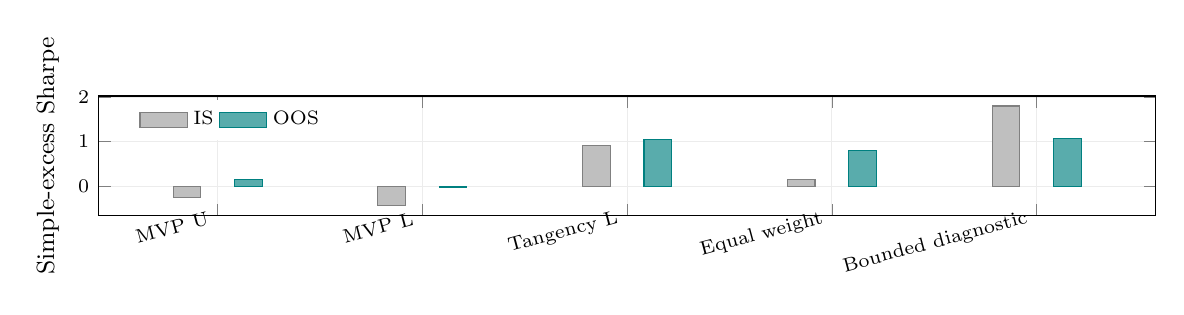
\begin{tikzpicture}\begin{axis}[width=15cm,height=5.1cm,tick label style={font=\scriptsize},label style={font=\small},legend style={font=\scriptsize,draw=none},scaled ticks=false,grid=major,grid style={gray!15},height=3.1cm,ylabel={Simple-excess Sharpe},xtick={0,1,2,3,4},xticklabels={MVP U,MVP L,Tangency L,Equal weight,Bounded diagnostic},x tick label style={font=\scriptsize,rotate=15,anchor=east},legend columns=2,legend pos=north west]
\addplot[ybar,area legend,bar shift=0pt,bar width=10pt,fill=gray!50,draw=gray] coordinates {(-0.150000,-0.263037) (0.850000,-0.436648) (1.850000,0.917358) (2.850000,0.153150) (3.850000,1.796878)};
\addlegendentry{IS}
\addplot[ybar,area legend,bar shift=0pt,bar width=10pt,fill=teal!65,draw=teal] coordinates {(0.150000,0.153683) (1.150000,-0.027496) (2.150000,1.052369) (3.150000,0.796231) (4.150000,1.059975)};
\addlegendentry{OOS}
\end{axis}\end{tikzpicture}
\captionof{figure}{In-sample versus held-out Sharpe, computed using the same simple-return convention in both periods.}\end{center}
\OOSInterpretation
\heading{5. Limitations and conclusion}
\textbf{Estimation and stability.} Historical means are imprecise, and highly correlated ETFs make optimized long--short allocations particularly sensitive to small changes in estimated returns. The full-sample frontier is descriptive, not a forecast: its weights use observations unavailable at the training cutoff. Covariance is also time-varying, so even an MVP fitted without mean estimates need not retain its predicted risk. The selected universe is not a random sample of all investable assets; conclusions are conditional on these ETFs and this window.

\textbf{Model and implementation.} Mean--variance analysis treats volatility as the risk criterion and does not separately penalize tail losses, illiquidity or margin calls. Weighted log means approximate, rather than equal, the growth of rebalanced wealth. Daily rebalancing ignores spreads, fees, taxes and turnover; leveraged portfolios additionally require financing and short-borrow assumptions. A per-position cap does not bound gross exposure, and a solvent frictionless wealth path does not establish that a strategy could meet real margin requirements. The severe drawdown of the bounded diagnostic illustrates why return and Sharpe should not be read in isolation.

\textbf{Evidence and practical conclusion.} The held-out comparison shows that the long-only tangency beats equal weight in Sharpe in this interval, but also incurs a deeper drawdown and concentrates in two assets. The MVPs achieve low realized volatility without superior Sharpe. Thus the results support a risk--return trade-off, not universal dominance of optimization over diversification. One chronological split has substantial sampling uncertainty and provides neither a confidence interval nor evidence that the ranking will persist.

A stronger assessment would use repeated rolling training/test windows, block-bootstrap uncertainty estimates, covariance shrinkage and mean regularization. Gross-leverage and turnover constraints, realistic borrowing costs and transaction-cost stress tests should then be imposed before considering implementation. Equal weight remains a transparent estimation-free benchmark; a constrained portfolio is justified only when its prospective risk budget and net-of-cost performance offer a defensible advantage.


\end{document}
